\chapter{Prenasal allophones of the front lax vowels}
\label{ch:prenasal}



This chapter presents the results of the GAMMs that were fit to the prenasal allophones of \trap, \dress, and \kit. First, I analyze \ban, \ben, and \bin in \S\ref{BAN}--\ref{BIN} and then I move to their pre-velar-nasal counterparts, \bang, \beng, and \bing in \S\ref{BANG}--\ref{BING}. A summary of findings regarding prenasal allophones in Cowlitz County and the prenasal split in general is found in \S\ref{sec:prenasal_discussion}. A more detailed discussion of how these patterns correlate to language-external effects in the region is found in Chapter~\ref{ch:discussion}.

\section{\ban}
\label{BAN}

In this sample there were 2,588 tokens of \ban coming from 402 unique words. The most common words were \textit{family}, \textit{man}, \textit{grandma}, \textit{understand}, \textit{camp}, \textit{hand}, \textit{grandpa}, \textit{Kalama}, and \textit{ran}. There was an average of 44 tokens per speaker\footnote{Speakers ranged from 15 to 104 tokens with a standard deviation of 19.2: 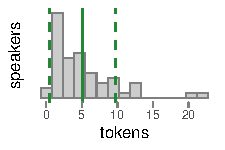
\includegraphics[width = 1.5in]{Figures/BANG/BANG_tiny.pdf}} and 324 per generation per sex. In Cowlitz County, the \ban vowel showed a number of large differences between social groups. Of the prenasal vowel classes, \ban was the one that I expected to exhibit the most social conditioning because of the patterns found in other communities in North American English. As this section will show, \ban was significantly affected by age and sex, putting Cowlitz County residents in line with other regions in the West.

\begin{figure*}[tb!]
    \centering
    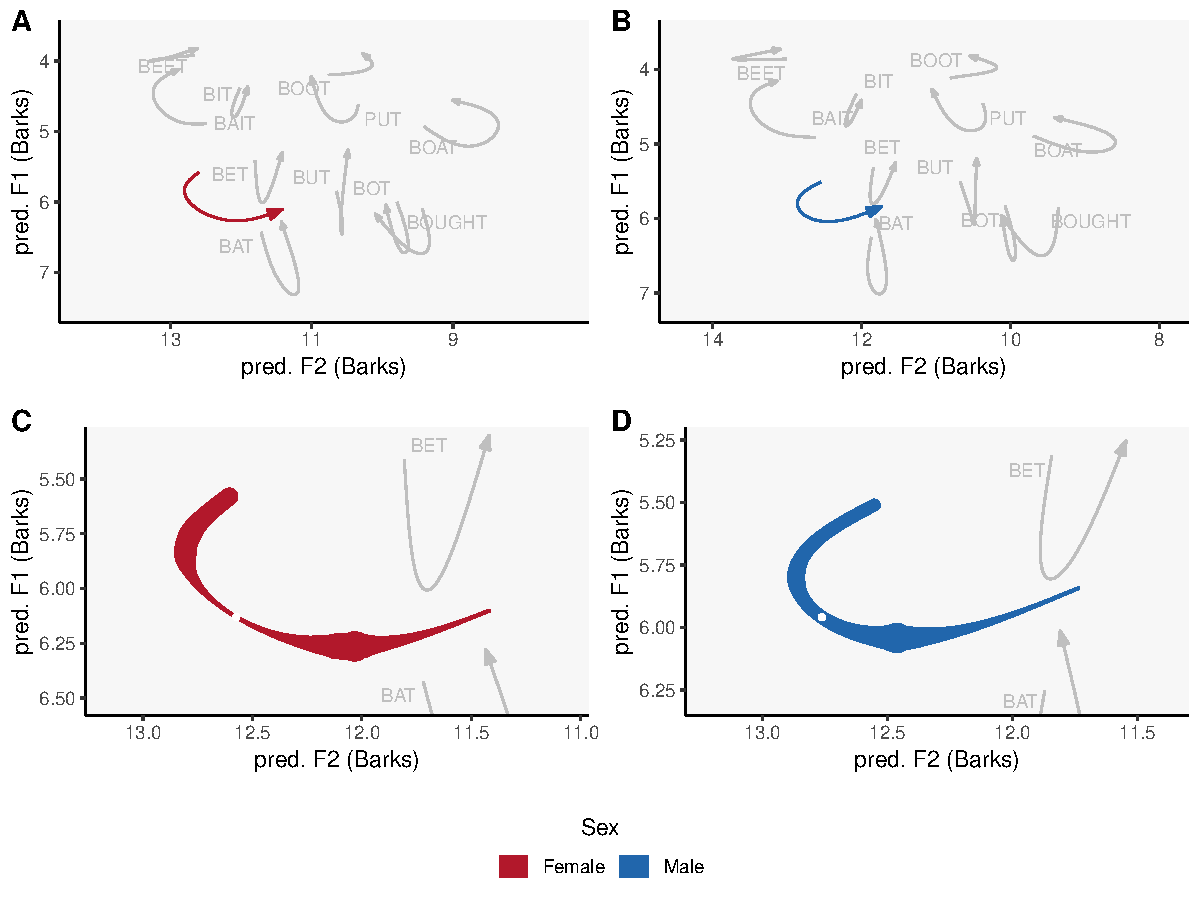
\includegraphics[width = 6.5in]{Figures/BAN/BAN_four_panel_plot_summarized.pdf}
    \caption[Predicted formant measurements for \ban by sex.]{Predicted formant measurements for \ban by sex with women on the left and men on the right. Predicted values are averaged across all generations.}
    \label{fig:BAN_four_panel_plot_summarized}
\end{figure*}

Figure~\ref{fig:BAN_four_panel_plot_summarized} provides a general view of \ban's trajectory. The first thing to notice is the shape of \ban's curve. Recall that \bat was ``pointy'': it lowered and backed during the first half of its trajectory, had a clear target as both formants reversed directions, and then raised and fronted slightly towards the offset. In contrast \ban is much smoother. From its relatively higher and fronter onset, the trajectory begins with a gradual raising of F1 and F2; at about 30\% into the duration of the vowel, F2 reverses and begins lowering (causing a front-most peak in the trajectory) while F1 continues to raise; at about two-thirds into the duration, F2 is still lowering but F1 reverses and begins lowering, causing the trajectory to move higher and backer in the vowel space until the offset. Put more simply, F1 and F2 both rise and then fall, but their peaks are not lined up. This is prototypical Bowl-shaped trajectory. An important consequence of this asynchrony (and a property of Bowls) is that the midpoint (the white dots in panels C and D of Figure~\ref{fig:BAN_four_panel_plot_summarized}) are somewhat meaningless as they capture neither the frontest nor the lowest points of the trajectory. In fact, because \ban is quite dynamic throughout its entire duration, no single measurement can adequately capture its trajectory.

In addition to its general shape, these plots show that \ban is indeed raised in Cowlitz County. For both sexes, the vowel space occupied by these trajectories do not overlap at all with those of \bat. In fact, \ban is about the same height, though quite a bit more fronted, as \bet. Thus, a more accurate transcription of this vowel is fronted, nasalized mid-open front vowel with a lowered, nasalized mid-open offglide: [\textipa{\t{\|+{\~E}\textsubarch{\|`{\~E}}}}].

This description of \ban by Cowlitz County speakers matches closely with \citeauthor{swan_2016_proceedings}'s \citeyearpar[10--12]{swan_2016_proceedings} detailed account of the trajectory of \ban in the Pacific Northwest. The speakers from Seattle, who had a more raised variant than the those from Vancouver, began \ban relatively high and front in the vowel space, peaking in frontness about a third of the way though, and gradually lowered with significant backing along the course of its duration before raising again at some point during the last third of its trajectory. The similarity between these two communities is striking and hints at some uniformity across the state with regards to \ban.

\begin{figure*}[tb!]
	\centering
	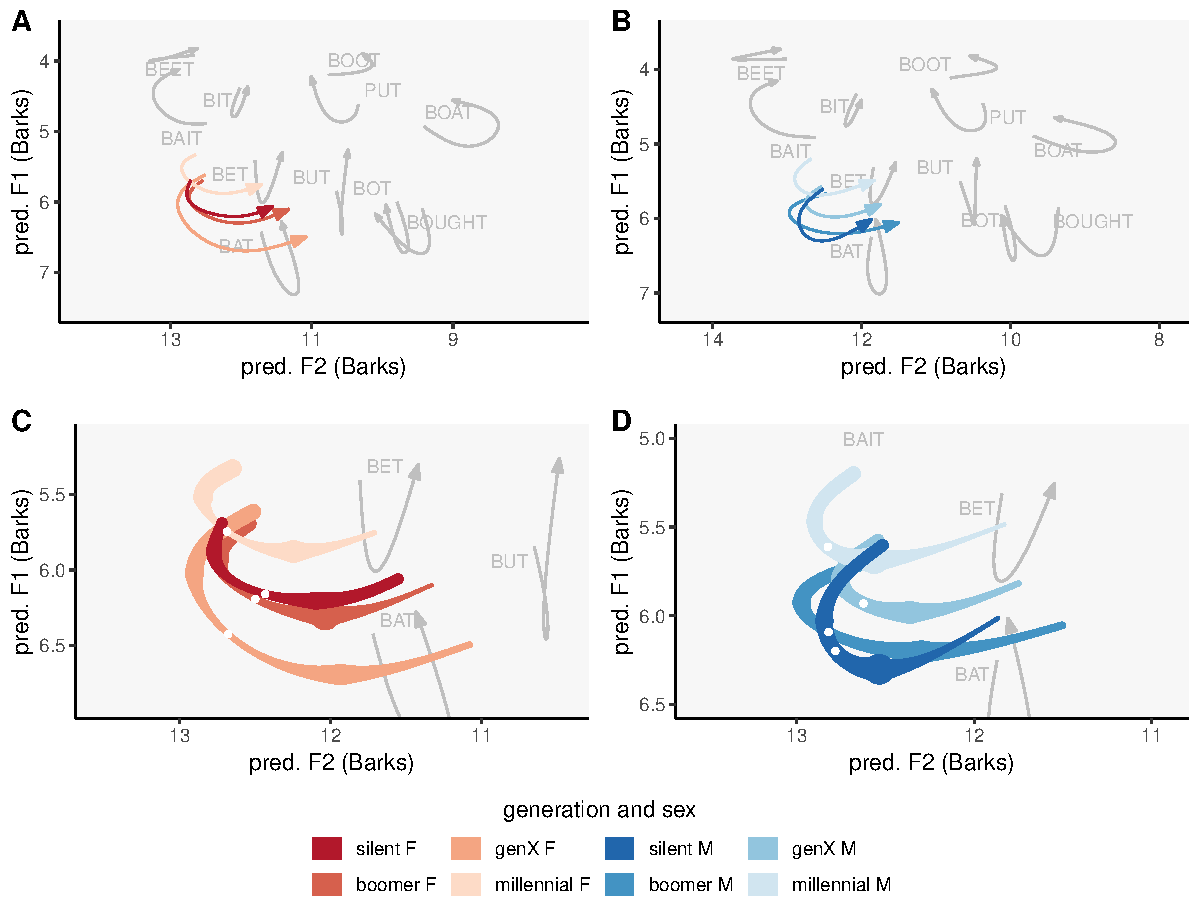
\includegraphics[width = 6.5in]{Figures/BAN/BAN_four_panel_plot.pdf}
	\caption[Predicted formant measurements for \ban by sex and generation.]{Predicted formant measurements for \ban by sex and generation. Women are on the left and men on the right. Darker shades represent older generations.}
	\label{fig:BAN_four_panel}
\end{figure*}

To visualize the effects of age on \ban, Figure~\ref{fig:BAN_four_panel} augments the curves plotted in Figure~\ref{fig:BAN_four_panel_plot_summarized} with additional trajectories for younger and older groups, illustrating two intriguing changes in apparent time. Beginning with the women, we see a unique reversal in the direction of language change. The oldest generation has a relatively high \ban, about as high as \bet but fronter. The Baby Boomer women were negligibly lower then the women in the Silent Generation (Appendix~\ref{appendix:difference_smooths}, Figure~\ref{fig:ban_diff_smooths_gen}A), suggesting that there was no change in this vowel before the 1960s. However, the women in Gen X used significantly lower and more diphthongal variants of \ban than the older two generations. Importantly, the bulk of this movement occurs during the offglide (namely the last third of the vowel's duration), while the onset is remaining stationary. As all of these plots do, panel C of Figure~\ref{fig:BAN_four_panel_plot_summarized} indicate the spectral rate of change with the thickness of the lines. Despite being a more dynamic vowel overall, the women in Gen X continue to spend a large amount of the duration of the vowel in the higher, fronter position before dropping down towards the offset, which also has the effect of pulling the midpoint towards the front (as evidenced by the thicker lines in panel C and the leftward shifting white dot).

This unusual pattern by the women in Gen X is supported in the raw formant measurements. Figure~\ref{fig:kim_prenasal} shows the average trajectories used by Kim, a woman born in 1968. Kim's \ban vowel is drastically more diphthongal than her other prenasal vowels with a trajectory length\footnote{Because this calculation is based in raw data, the trajectory length is calculated by taking the sum of the euclidean distances between the 11 time points from which formants were extracted. These measurements are based on Bark-transformed normalized data.} of a staggering 4.10 Barks. Figure~\ref{fig:holly_prenasal} shows another woman from Gen X who has a variant of \ban that is quite diphthongal (though not as extreme as Kim's) with a modest trajectory length of 3.26 Barks.

\begin{figure*}[tb!]
    \centering
    \hspace{\fill}
    \begin{subfigure}[t]{2.925in}
        \centering
        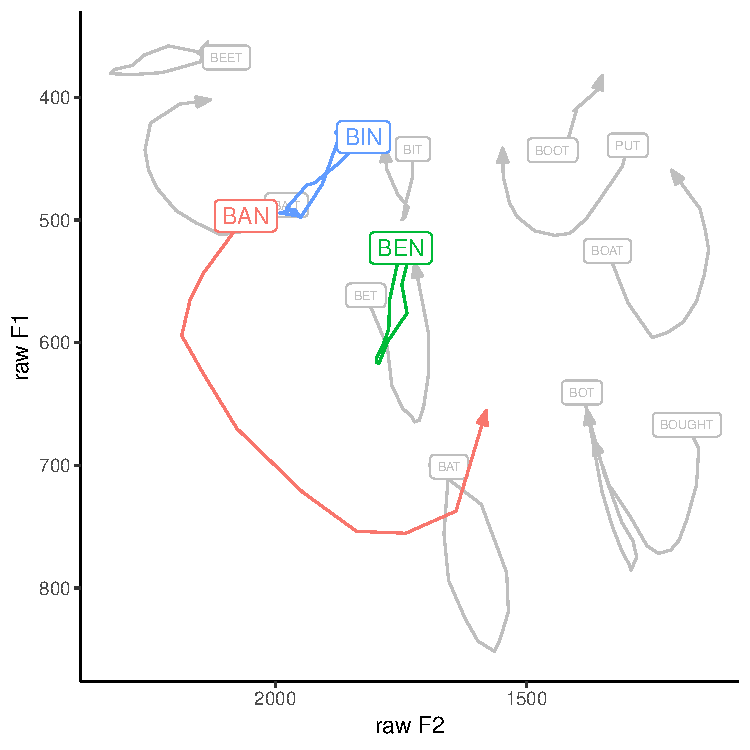
\includegraphics[width = \textwidth]{Figures/example_plots/24-Kim_avg_prenasal.pdf}
        \caption{Kim's prenasal vowels.}
        \label{fig:kim_prenasal}
    \end{subfigure}
    \hspace{\fill}
    \begin{subfigure}[t]{2.925in}
        \centering
        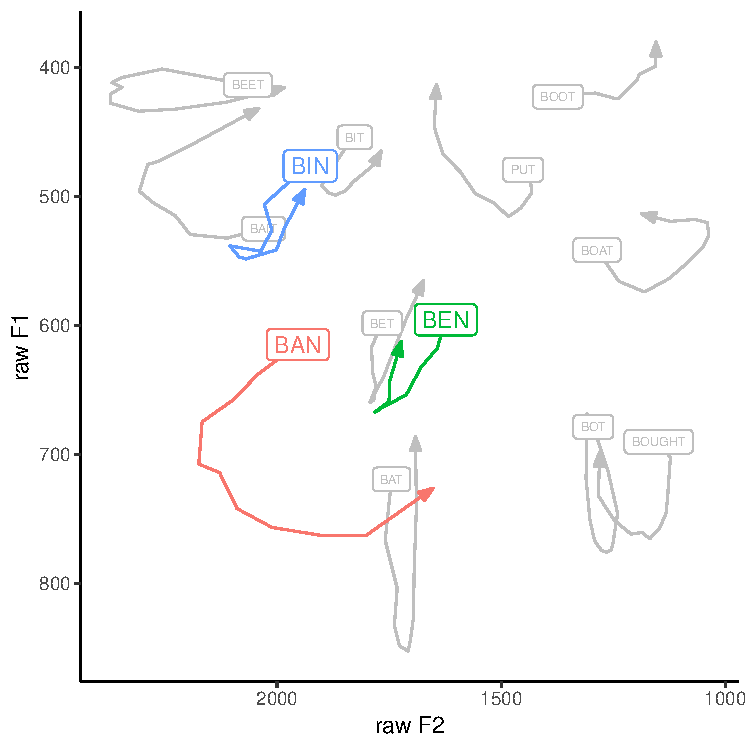
\includegraphics[width = \textwidth]{Figures/example_plots/48-Holly_avg_prenasal.pdf}
        \caption{Holly's prenasal vowels.}
        \label{fig:holly_prenasal}
    \end{subfigure}
    \hspace{\fill}
    \caption{Average trajectories (in normalized Hz) for two women in Gen X showing the diphthongal \ban vowel.}
    \label{fig:kim_and_holly}
\end{figure*}

This lowering by the women in Gen X drastically reverses when the Millennial women are added to the picture. These youngest speakers have a much higher realization of \ban---even higher than the Silent women. It was also quite a bit more monophthongal too: the trajectory length in the oldest two generations averaged was 1.75 Barks, in Gen X it was 2.72 Barks, and in the Millennials it was 1.57 Barks. So in this sample we see a pattern of stability, followed by lowering and diphthongization, and then followed by raising and monophthongization.

While the women undergo change in one direction with a quick reversal by the Millennials, the men appear to gradually raise \ban over the four generations. The right panels of Figure~\ref{fig:BAN_four_panel_plot_summarized} show the men's predicted trajectories in shades of blue, with the oldest generation in the darkest shade. In stark contrast to the women's pattern, the oldest men had the lowest realization of \ban. And while women were stable or lowering \ban, this data suggests that the men were gradually raising it. This leads to the youngest generation which, like the women, have the highest variants of \ban. The difference smooths suggest no statistically significant amount of raising between any consecutive generation of men (\ref{fig:ban_diff_smooths_gen}C--D,O--P,W--X), but when the oldest two generations are compared to the Millennials, the latter 50\%--75\% of the trajectory is significantly higher (\ref{fig:ban_diff_smooths_gen}K,S). Furthermore, while the women had a Bowl-shaped \ban, the men appear to have a wide U instead since the midpoint is more prominent, and there is little indication of two targets like among the women.

\begin{figure*}[p]
	\centering
	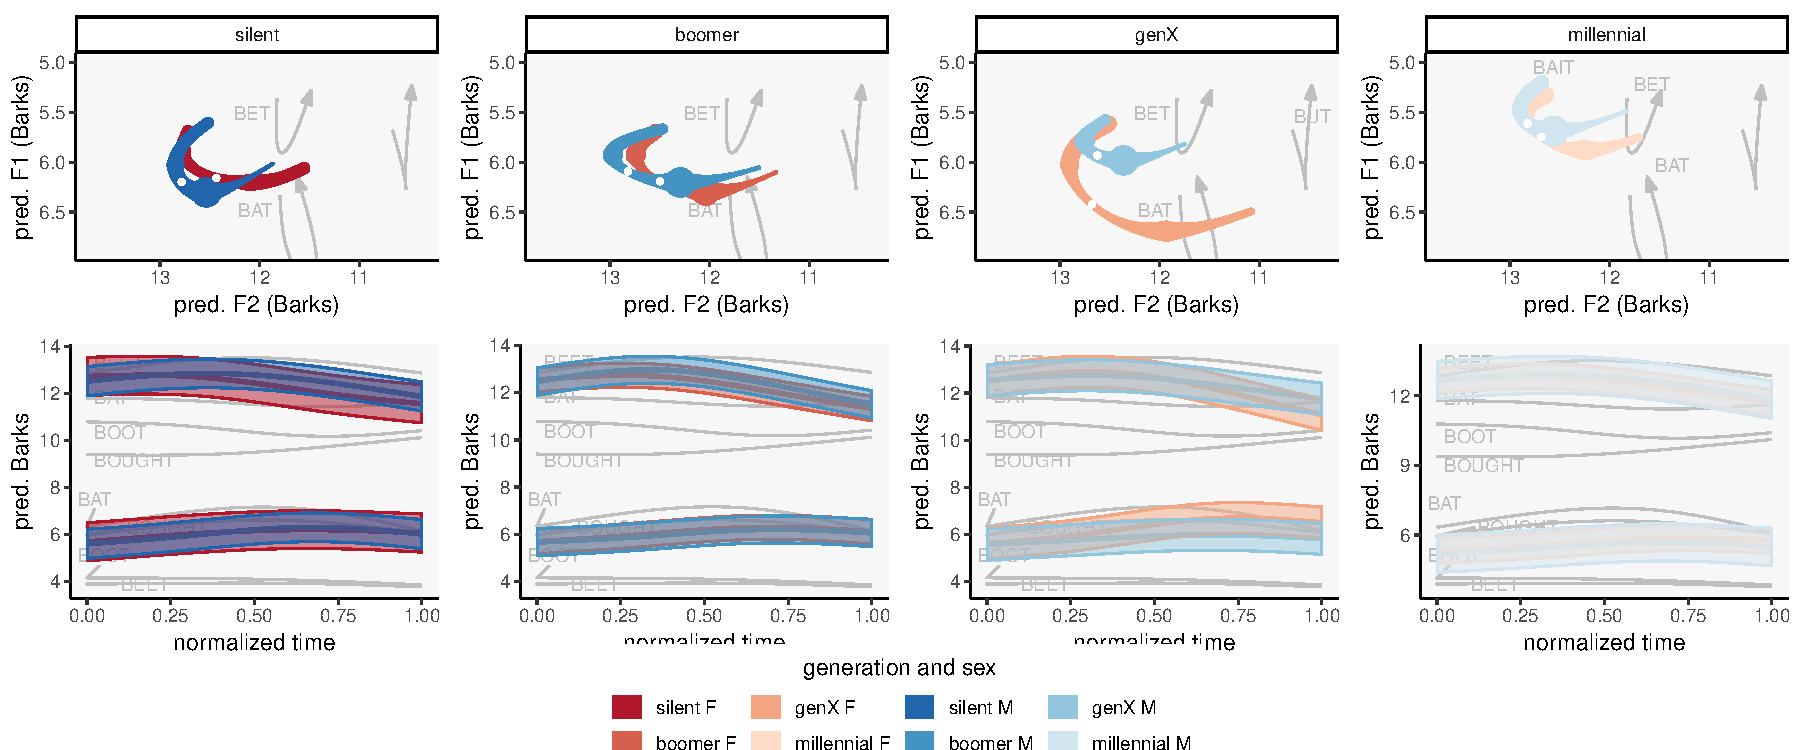
\includegraphics[angle = 90, origin = c, height = 6in]{Figures/BAN/BAN_sex_panel_plot_wide.pdf}
	\caption[Predicted formant measurements for \ban by generation.]{Predicted formant measurements for \ban by generation.}
	\label{fig:BAN_sex_panel_plot_wide}
\end{figure*}

By examining the generations one at a time and comparing the sexes within them, as in Figure~\ref{fig:BAN_sex_panel_plot_wide}, we see additional support for the two patterns described above. In the Silent and Baby Boomer generations, the difference smooths show very little difference (\ref{fig:ban_diff_smooths_sex_gen}A--D). This sameness between the sexes coupled with no change across generations for both men and women suggests relative stability for the first two generations and that \ban was not undergoing language change at this time. But with Gen X, the men begin to raise \ban and the women lower it, resulting very large difference between the sexes in the second half of the vowel's trajectory (\ref{fig:ban_diff_smooths_sex_gen}E--F). Finally, the Millennial women raise \ban to catch up with the men, resulting in no statistically significant differences between them (\ref{fig:ban_diff_smooths_sex_gen}G--H). Other than Gen X, the two sexes are approximately the same in the four generations represented in this sample.

Summarizing \ban, we see that the general shape of \ban is similar to realizations recorded in Seattle (a Bowl for the women and a wide U for the men) and that the primary dimension of change is in F1. With the exception of the women in Gen X, the overall pattern was that of raising. Women began lowering \ban in Gen X but then the Millennial-aged speakers raised it considerably. The men progressively raised \ban across all four generations.






\section{\ben}
\label{BEN}

In this dataset there were 4,445 tokens of \ben coming from 375 unique words. The most common words were \textit{went}, \textit{remember}, \textit{anything}, \textit{anyway}, \textit{ten}, \textit{many}, \textit{end(ed)}, \textit{twenty}, \textit{friend(s)}, and \textit{spent}. There was an average of 82 tokens per speaker\footnote{Speakers ranged from 23 to 250 tokens with a standard deviation of 36.4: 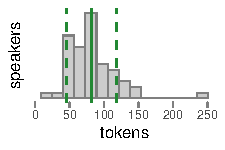
\includegraphics[width = 1.5in]{Figures/BEN/BEN_tiny.pdf}} and 556 per generation per sex. Like \ban, there are significant social effects that condition the realization of \ben, though this is primarily restricted to the women in this Cowlitz County sample.

\begin{figure*}[tb!]
    \centering
    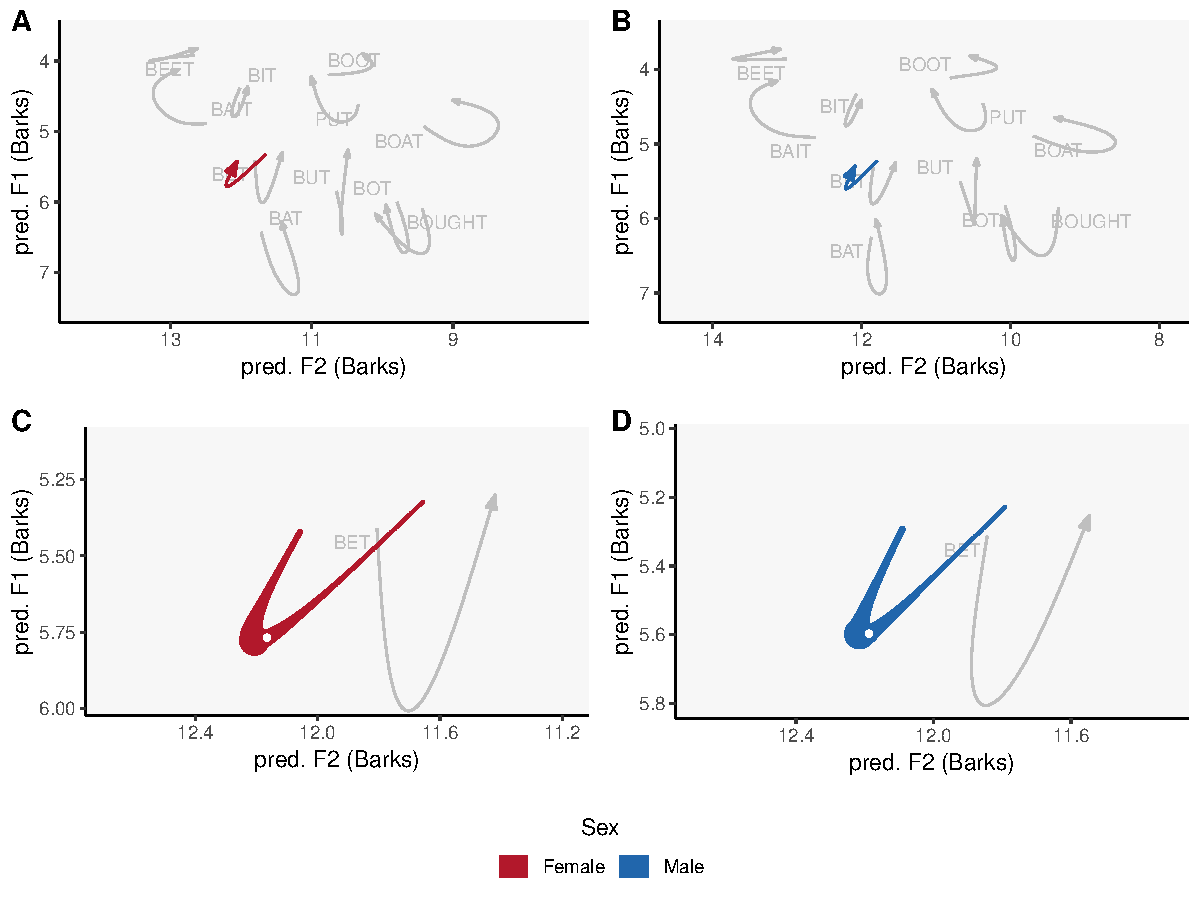
\includegraphics[width = 6.5in]{Figures/BEN/BEN_four_panel_plot_summarized.pdf}
    \caption[Predicted formant measurements for \ben by sex.]{Predicted formant measurements for \ben by sex with women on the left and men on the right. Predicted values are averaged across all generations.}
    \label{fig:BEN_four_panel_plot_summarized}
\end{figure*}

Figure~\ref{fig:BEN_four_panel_plot_summarized} shows the effect of sex of \ben. There is relatively little difference between the sexes as far as relative position of the vowel or its shape, but its direction and shape are markedly different from the \ban (or \bin for that matter). Most notably, the offset is fronter than its onset, meaning this vowel is not ingliding as \bet is. As for its shape, as described previously, \ban has a characteristically smooth shape caused by the asynchrony of when F1 and F2 reverse directions. In stark contrast, \ben had a much pointier curve with the changes in F1 and F2 much more closely aligned, resulting in a V. The vowel starts very near where \bet starts, but it lowers and fronts to its target, which is slightly fronter than \bet. After reaching its target, it reverses directions raises and retracts slightly towards if offset. Because of this vowel's clear target and relatively little movement in the F1-F2 space, I would consider this a fronted, nasalized, mid front lax monophthong, transcribed as [\textipa{\~{\|+E}}].

\begin{figure*}[tb!]
	\centering
	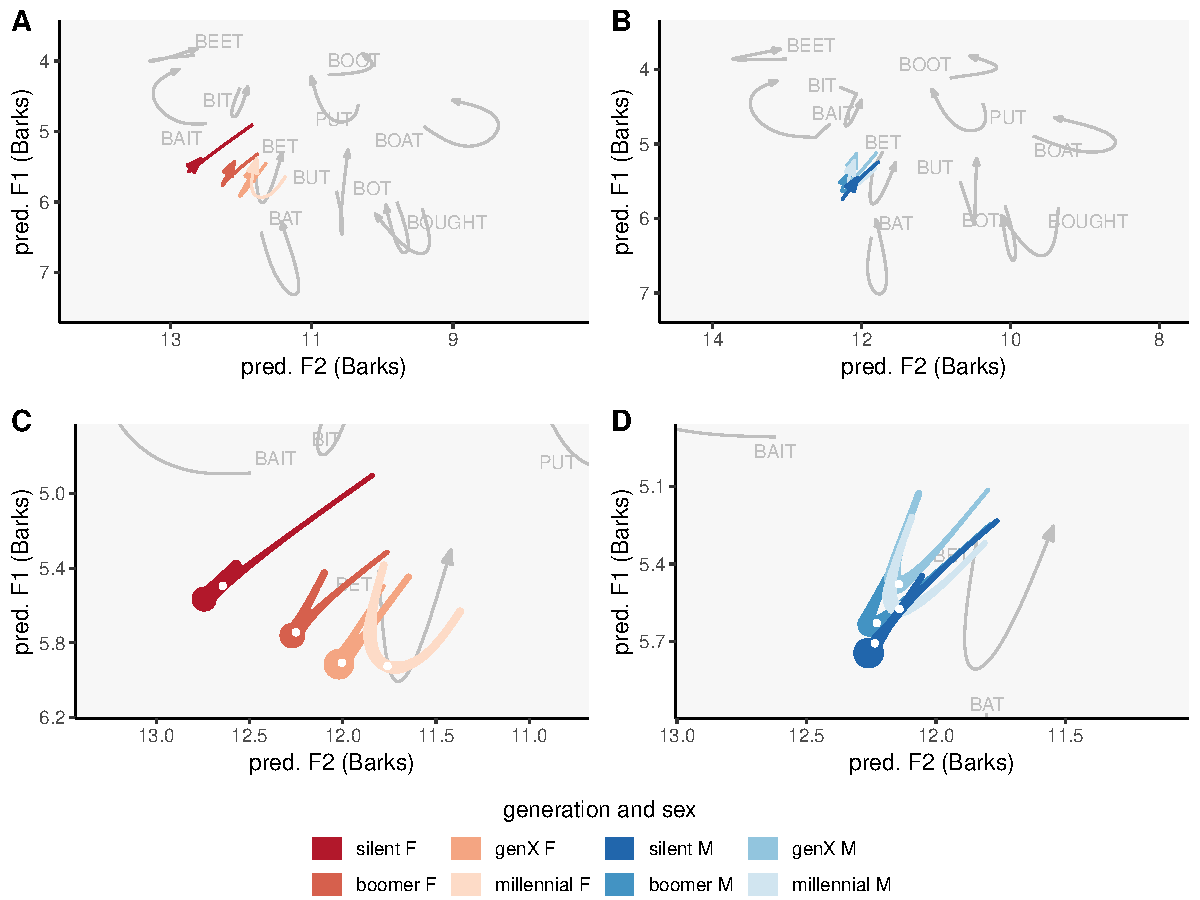
\includegraphics[width = 6.5in]{Figures/BEN/BEN_four_panel_plot.pdf}
	\caption[Predicted formant measurements for \ben by sex and generation.]{Predicted formant measurements for \ben by sex and generation. Women are on the left and men on the right. Darker shades represent older generations.}
	\label{fig:BEN_four_panel}
\end{figure*}

The interpretation of this vowel is complicated slightly when the data is split by generation, as in Figure~\ref{fig:BEN_four_panel}. On the left, the women are clearly backing and slightly lowering the vowel in apparent time. The women of the Silent Generation had quite a fronted and raised variant of \ben but then the next two generations gradually retracted and lowered it.\footnote{Difference smooths suggest that this lowering happened primarily between the Silent Generation and the Baby Boomers (\ref{fig:ben_diff_smooths_gen}A).} Figure~\ref{fig:ben_diff_smooths_gen} in Appendix~\ref{appendix:difference_smooths} shows the difference smooths for these predicted values and suggests that the primary axis of change, which is statistically significant and relatively large, is along the F2 dimension (\ref{fig:ben_diff_smooths_gen}B,F,J,N,R). With each successive generation of women, the vowel was more centralized, to the point that the confidence intervals for the GAMM did not overlap for over half of the vowels' trajectory. Comparing non-adjacent generations only increases the differences. In fact, there was no overlap between the Millennial women's F2 in \ben and either the Baby Boomers' (\ref{fig:ben_diff_smooths_gen}R) or the women in the Silent Generation (\ref{fig:ben_diff_smooths_gen}J). So, it appears to be the case that \ben-retraction is robust in the women of this community and has been progressing actively for several generations. Meanwhile, there is some indication of \ben lowering in apparent time, but it was not as strong as the retraction. The difference between successive generations was not statistically significant in F1 (\ref{fig:ben_diff_smooths_gen}M,U), so it does not appear to be the case that children acquired a markedly different realization of \ben than their parents, at least in vowel height. However, when comparing the Silent with the Boomers and Gen X, there is a meaningful difference in the first half of the trajectory (\ref{fig:ben_diff_smooths_gen}A). Summarizing the movement of \ben in apparent time and the vowel space, a woman's \ben is more retracted than her mother's and more retracted and lower than her grandmother's.

In addition to their continued retraction, the Millennial women also drastically change the shape of the curve; the vowel's Bounce or V-shape is no longer present in the Millennial women's \bet and the changes in F1 and F2 are less abrupt, resulting in a U-shaped pattern akin to \bet.

There is one more change that makes \ben stand out compared to the other vowels in this study: the time point of the peak F1. The women in the Silent generation achieve the highest F1 two-thirds into the vowel's duration. This is somewhat evident in panel C of Figure~\ref{fig:BEN_four_panel} where the white dot representing the midpoint does not line up with the vowel's target.\footnote{This can also be seen in the spectrogram-like portion of the plots in Figure  (\ref{fig:ben_diff_smooths_gen}).} With each successive generation, this peak F1 shifts closer to the onset, such that the Millennial women's maximum F1 was about 44\% into the vowel's duration.\footnote{These numbers were found by extracting 501 points from the predicted trajectories of \ben for each generation and finding the time point that had the maximum F1.} So not only do the women lower, retract, and change the vowel's shape, but they are also altering when this nucleus is achieved.

For the men, there is little change. All four generations have very similar realizations of \ben that are in nearly identical positions in the vowel space, slightly fronter than \bet. Comparing the older three generations, there is a slight pattern of \ben raising in apparent time, with the Millennial men breaking the trend and lowering the vowel. The Millennial men also appear to have lost some of the pointiness to their curve and join their female cohorts in a more U-shaped pattern. Also, just like the women, the peak F1 also shifts earlier along the vowel's duration. However, the pairwise difference smooths between generations suggests no significant difference in either F1 or F2 between any two generations of men for \ben,\footnote{The one exception to this is the last third of the F1 differences between Silent men and Gen X men (\ref{fig:ben_diff_smooths_gen}G but I'm reluctant to call this a meaningful change.} so the differences, even spanning multiple generations, are small (\ref{fig:ben_diff_smooths_gen}, right two columns). Overall, Figure~\ref{fig:BEN_four_panel} shows that the men are largely immune from the changes happening in the women's speech.

\begin{figure*}[p]
	\centering
	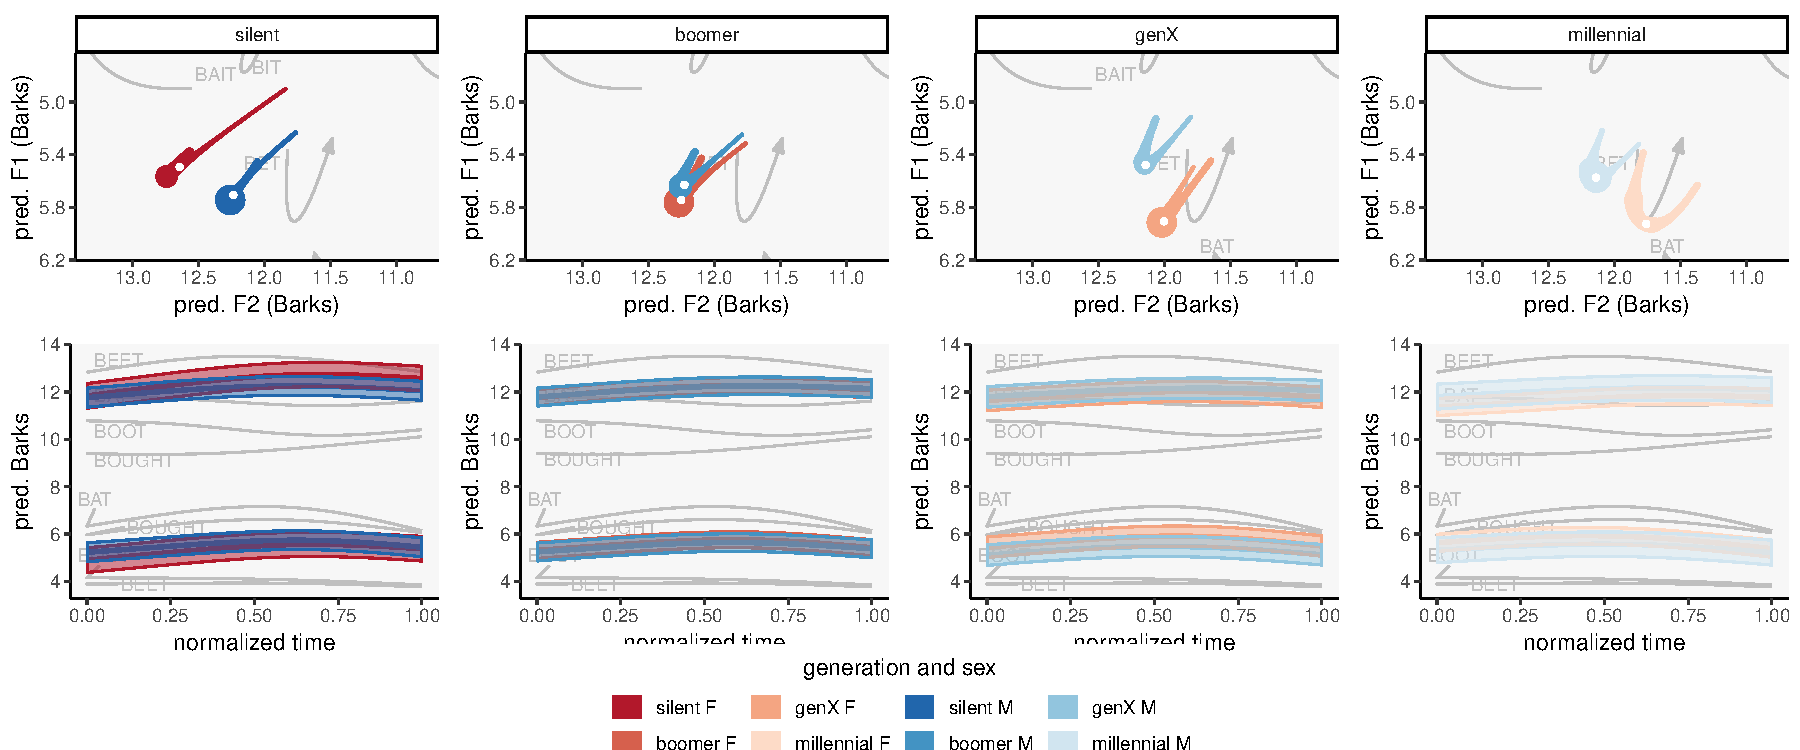
\includegraphics[angle = 90, origin = c, height = 6in]{Figures/BEN/BEN_sex_panel_plot_wide.pdf}
	\caption[Predicted formant measurements for \ben by generation.]{Predicted formant measurements for \ben by generation.}
	\label{fig:BEN_sex_panel_plot_wide}
\end{figure*}

When generations are isolated, as in Figure~\ref{fig:BEN_sex_panel_plot_wide}, the amount of shifting in the women and the stability in the men becomes more apparent. In the Silent Generation, the women use more fronted variants (\ref{fig:ben_diff_smooths_sex_gen}B). In the Boomers, difference smooths suggest no statistical significance (\ref{fig:ben_diff_smooths_sex_gen}C--D). But this similarity does not suggest the end of a shift because the women continue to lower and retract, and the difference smooths show almost no overlap in F1 between the two sexes (\ref{fig:ben_diff_smooths_sex_gen}E). Finally, with the Millennials, the women are more centralized compared to the men (the F2 difference smooth was statistically significant for its entire duration; \ref{fig:ben_diff_smooths_sex_gen}H) and quite a bit lower (F1 was lower for the first two-thirds of the trajectory; \ref{fig:ben_diff_smooths_sex_gen}G). In essence, Figure~\ref{fig:BEN_sex_panel_plot_wide} shows that the men are relatively stable during the four generations here, but that women quickly shift past them. The question that remains then is why the sexes were so different in the Silent Generation. For now I leave this pattern in the Silent Generation as open question and hope that future research will help address this pattern.

The last thing that Figure~\ref{fig:BEN_sex_panel_plot_wide} illustrates (better than Figure~\ref{fig:BEN_four_panel} at least) is that the sexes had roughly similar trajectory shapes within generations. Specifically, the oldest generation has a ``point'' shaped trajectory, but over time, it becomes more U-like. Recall that this was also found with \bet, that even though the women steadily advanced their shift of the vowel, the shape of the men's vowel was remarkably similar as the women's. Again, this is not a product of the model because each combination of sex and generation was included as independent factor levels. It is even more remarkable that a finding that was unique to \bet is also found for \ben. Thus it appears that there is some sort of pattern associated with \dress such that the men shift their trajectories in step with the women, but not the position of the vowel.

Summarizing \ben, this section showed that \ben were very different in shape than other prenasal tokens. To my knowledge, there is no detailed description of \ben in literature on Western English, so it is unclear whether these patterns are unique trends to this community or if they can be found more broadly in the West. Regardless, the position of \ben changes in apparent time for the women, with younger generation successively lowering and retracting the vowel. However, both sexes smooth the trajectory out at the same time, going from a pointed shape to a U-shape.



\section{\bin}
\label{BIN}

The \bin vowel is defined as tokens of \bit before /\textipa{m}/ or /\textipa{n}/. In this corpus, there were 1,563 tokens of \bin coming from 265 unique words. The most common words were \textit{interesting}, \textit{since}, \textit{minutes}, \textit{timber}, \textit{dinner}, \textit{industry}, \textit{finished}, \textit{swimming}, \textit{cinnamon}, and \textit{inch}. In conversation, there was an average of 29 tokens per speaker\footnote{Speakers ranged from 5 to 72 tokens with a standard deviation of 12.3: 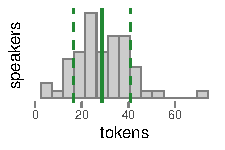
\includegraphics[width = 1.5in]{Figures/BIN/BIN_tiny.pdf}} and 195 per generation per sex. Compared to \ban and \ben, there is relatively little variation in \bin in Cowlitz County.

\begin{figure*}[tb!]
    \centering
    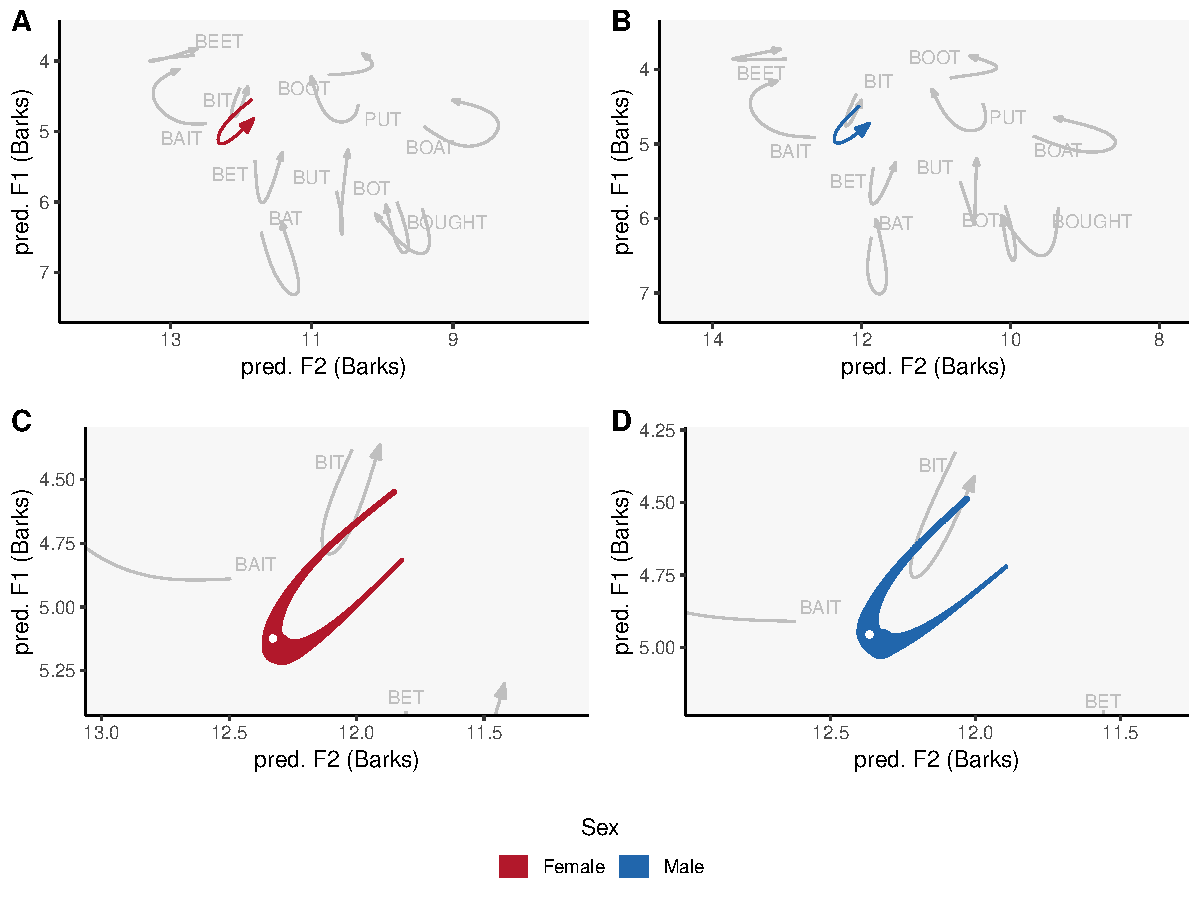
\includegraphics[width = 6.5in]{Figures/BIN/BIN_four_panel_plot_summarized.pdf}
    \caption[Predicted formant measurements for \bin by sex.]{Predicted formant measurements for \bin by sex with women on the left and men on the right. Predicted values are averaged across all generations.}
    \label{fig:BIN_four_panel_plot_summarized}
\end{figure*}

Figure~\ref{fig:BIN_four_panel_plot_summarized} shows the overall shape of \bin and its position in the vowel space. The shape of this vowel's trajectory is similar to \ban: its U-shaped curve is caused by gradual changes in F1 and F2, with its lowest and frontest point being achieved about halfway into the vowel's duration. Overall the vowel does not traverse through much of the F1-F2 space,\footnote{Its trajectory length was 1.29 Barks. For reference, \ben was more monophthongal on average at 1.01 Barks and \ban was more diphthongal at 1.80 Barks.} making it a relatively monophthongal, lowered, nasalized, high front lax vowel: [\textipa{\~{\|`I}}]. Continuing with the trend set by \ban and \ben, \bin is also fronter than its non-nasal counterpart. However, unlike \ban and \ben, \bin is actually lower in the vowel space than its corresponding elsewhere allophone, \bit.

\begin{figure*}[tb!]
	\centering
	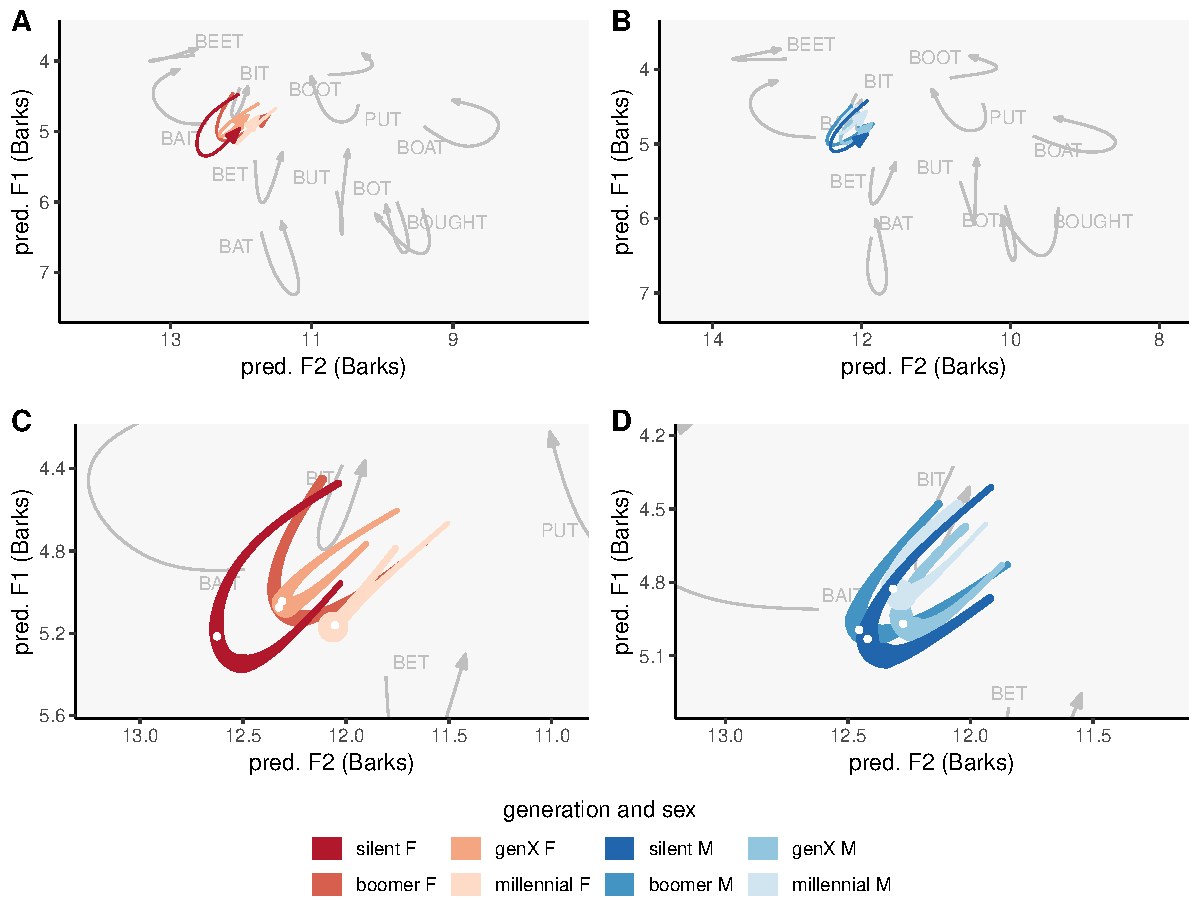
\includegraphics[width = 6.5in]{Figures/BIN/BIN_four_panel_plot.pdf}
	\caption[Predicted formant measurements for \bin by sex and generation.]{Predicted formant measurements for \bin by sex and generation. Women are on the left and men on the right. Darker shades represent older generations.}
	\label{fig:BIN_four_panel}
\end{figure*}

Figure~\ref{fig:BIN_four_panel} shows how this realization changes in apparent time by sex. On the left, panels A and C indicate retraction and a change in the shape of \bin across the four generations of women. The oldest women had the most fronted and most dynamic variant of \bin. The realizations used by the Boomer women were more or less the same as those by the Silent women only slightly retracted, though this difference was significant only at the very end of the vowel's duration (\ref{fig:bin_diff_smooths_gen}B). The Gen X women's realizations were approximately in the same vowel space as the Boomers, but the vowel became less dynamic and developed a clearer nucleus; this difference between the middle generations was only significant in the portions closest to the onset and offset of the vowel, suggesting a change in shape more than a change in position (\ref{fig:bin_diff_smooths_gen}N). Finally, the Millennial women continued the trend and used the most centralized, the least dynamic,\footnote{The trajectory length in Barks for the Millennial women's \bin was 0.95 while the Silent women's was a full 50\% longer at 1.43.} and the pointiest variant of \bin. These changes with the Millennial women were significantly different from all three older generations of women, particularly in the first half of the vowel's duration in the F2 measurements (\ref{fig:bin_diff_smooths_gen}J,R,V). However, panel A of Figure~\ref{fig:BIN_four_panel} shows that these changes all happen within a very small portion of the F1-F2 space. Like \bit, it appears then that the women are making small but significant changes to \bin by retracting it slightly and making the vowel less dynamic.

For the men, the pattern is similar to \bit: there is little evidence of change. Difference smooths show no statistically significant difference between any generation of the men's vowels at any point along their duration, for any pair of generations (\ref{fig:bin_diff_smooths_gen}, right two columns).

\begin{figure*}[p]
	\centering
	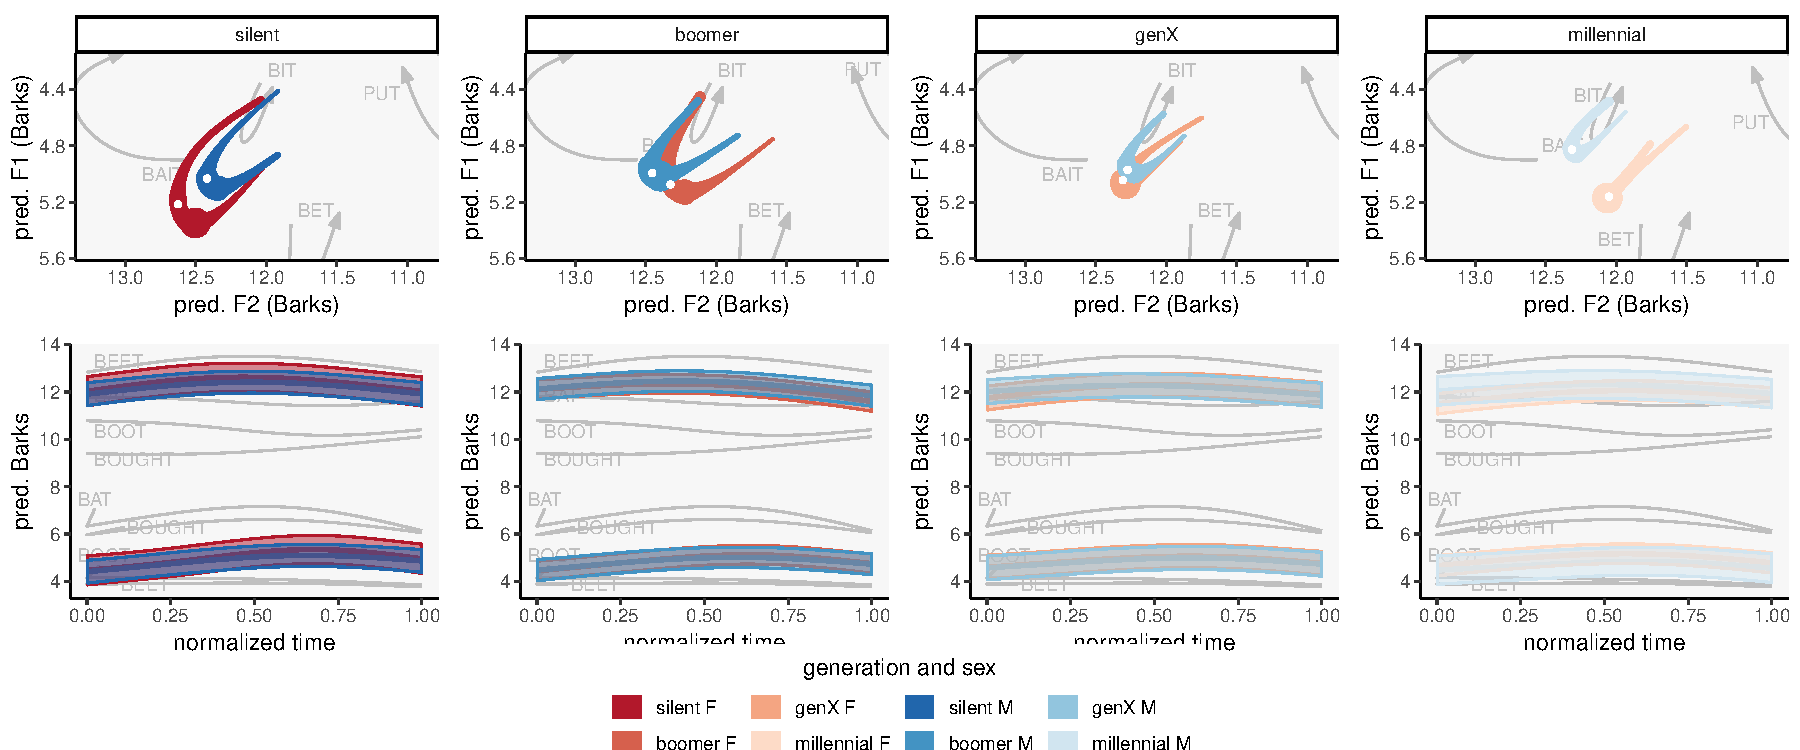
\includegraphics[angle = 90, origin = c, height = 6in]{Figures/BIN/BIN_sex_panel_plot_wide.pdf}
	\caption[Predicted formant measurements for \bin by generation.]{Predicted formant measurements for \bin by generation.}
	\label{fig:BIN_sex_panel_plot_wide}
\end{figure*}

Looking at \bin by generation, Figure~\ref{fig:BIN_sex_panel_plot_wide} shows that the differences between the sexes was relatively small. For the first three generations, difference smooths suggest no statistically significant difference between men and women (\ref{fig:bin_diff_smooths_sex_gen}A--F). However, visually, it appears that the men's shape for \bin approximately matches the women's. Thus we have a bit of a paradox: the women show signs of change but the men do not, yet between the two groups there is no difference. This may simply be the result of the women's changes being so small in the vowel space. However, when the Millennials are examined, we see that the women's realizations are statistically lower during the middle half of the vowel (\ref{fig:bin_diff_smooths_sex_gen}G), and more retracted during the first 40\% (\ref{fig:bin_diff_smooths_sex_gen}H). Thus we have a situation where there is relative stability for three generations, with the only change being in the shape of the vowel's trajectory, but then the Millennial women suddenly begin lowering and retracting the vowel.

Finally, the most visible change across time is in the shape of the formant trajectories. The oldest generation realized \bin with a U-shape; the women's curve may even be considered a Bowl. Over the next three generations, the curve narrows to the point of becoming a prototypical Bounce in the Millennial women. Among the men, the change is not so drastic since the Lost men's \bin is not quite so dynamic and the Millennial men's \bin is not quite a Bounce.

In summary, \bin was realized slightly lower than \bit and the shape of the vowel was generally U-shaped, like \ban, though it was much less dynamic and was contained a relatively small portion of the vowel space. For the women, there was a small but significant indication of retraction and monophthongization in apparent time with the Millennial women shifting the vowel the most. For the men, there was no evidence of change.

\section{Interim summary}

So far, this chapter has described the patterns found in \ban, \ben, and \bin (the pre-/\textipa{m}/ and pre-/\textipa{n}/ tokens of \trap, \dress, and \kit). For \ban, both sexes gradually raised it with the exception of the Gen X women who lowered it. For \ben, the women lower and retract it while changing its shape. \bin did not lower but the women appear to retract it by a small amount. Thus we see shifting in three different directions. There was no evidence of apparent time change in the position of men's realizations of \ben or \bin, but their curves became pointier. In many cases for both sexes, the vowel does not shift in the F1-F2 space, but instead it becomes more monophthongal.

The next three sections treat a different subset of prenasal tokens, \bang, \beng, and \bing, to identify changes that occur before pre-velar-nasal front lax vowels.








\section{\bang}
\label{BANG}

In this sample, there were 275 tokens of \bang coming from 56 unique words. The most common words were \textit{language}, \textit{thank(s)}, \textit{hang(ing)}, \textit{Da Nang},\footnote{Da Nang is a city in Vietnam that had a U.S. Air Force base during the Vietnam War. One speaker told stories of when he served there.} \textit{tank}, \textit{angry}, \textit{bank} and \textit{ankle}. There was an average of 5 tokens per person,\footnote{Of the speakers that produced any \bang tokens, they ranged from 1 to 22 tokens with a standard deviation of 37.1: 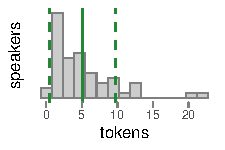
\includegraphics[width = 1.5in]{Figures/BANG/BANG_tiny.pdf} Two speakers, Laura (female Boomer) and Dale (male Silent), did not use any tokens of 10 \bang.} and 34 per generation per sex. This is admittedly not a lot of data to be working with, but the results of the GAMMs are reasonable and coincide with my intuitions of the data.

\begin{figure*}[tb!]
    \centering
    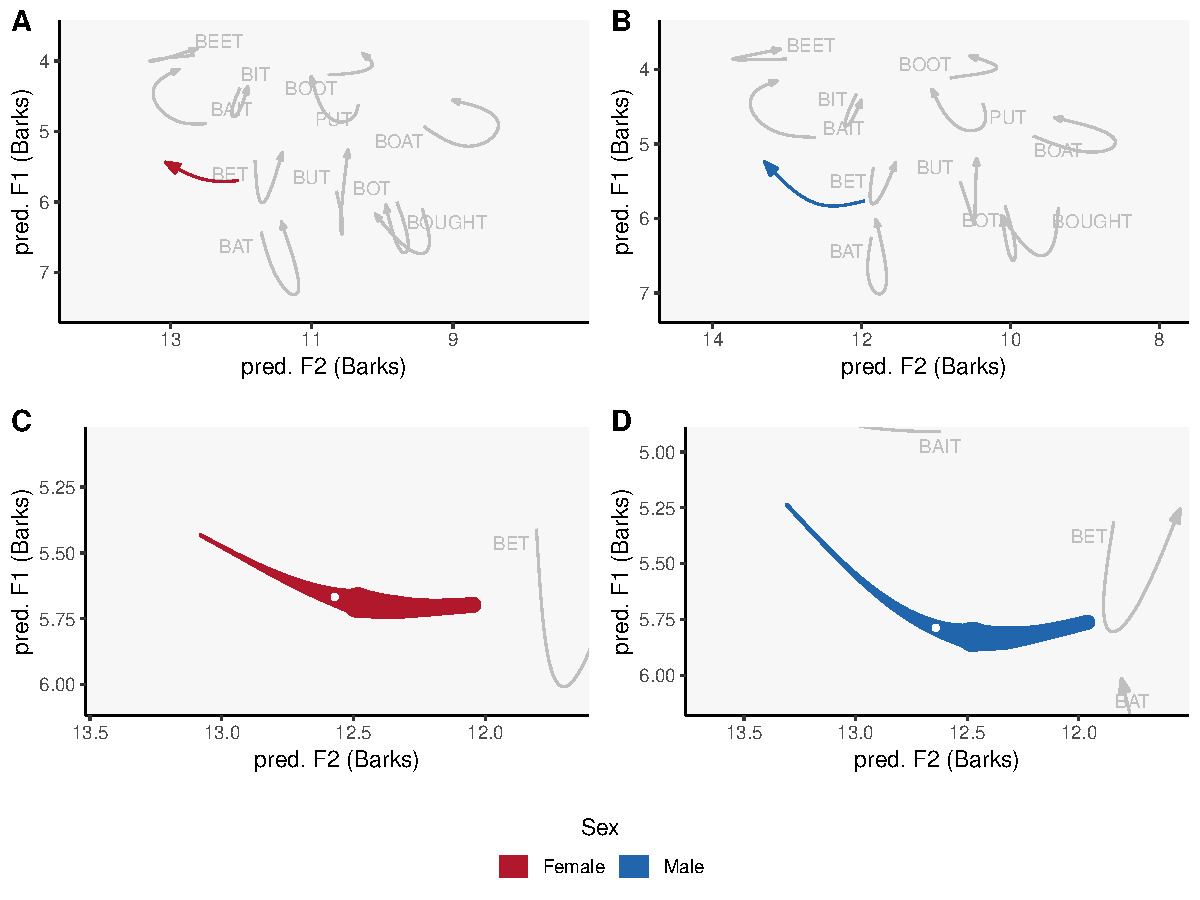
\includegraphics[width = 6.5in]{Figures/BANG/BANG_four_panel_plot_summarized.pdf}
    \caption[Predicted formant measurements for \bang by sex.]{Predicted formant measurements for \bang by sex with women on the left and men on the right. Predicted values are averaged across all generations.}
    \label{fig:BANG_four_panel_plot_summarized}
\end{figure*}

Figure~\ref{fig:BANG_four_panel_plot_summarized} show a general plot for \bang. First, it is clear that the shape of this vowel's trajectory is different from the others in that there is relatively little movement in F1 and that almost all of the change is in F2. This is a very wide U-shape, and is close to a prototypical Line-shaped trajectory. This raising is undoubtedly a result of the velar pinch, which causes a sharp rise in F2 as the back of the tongue raises to form the velar consonant. It is difficult to determine the precise target for this vowel since there is no real steady state. Not only does this make any one measurement somewhat arbitrary, it suggests that this vowel may be characterized by the overall position and shape of its trajectory rather than by a single point in the vowel space. Transcribed into IPA, this vowel is [\textipa{\t{\~E\textsubarch{\|+{\|'{\~E}}}}}]\vspace{-0.35em}, a nasalized mid-open diphthong, with a raised and fronted offglide.
% Nice hack to correct the extra line spacing when the stacked diacritics adjusted the baseline height. 0.35em is just eyeballing it and it looks pretty good even when zoomed way in.

\begin{figure*}[tb!]
	\centering
	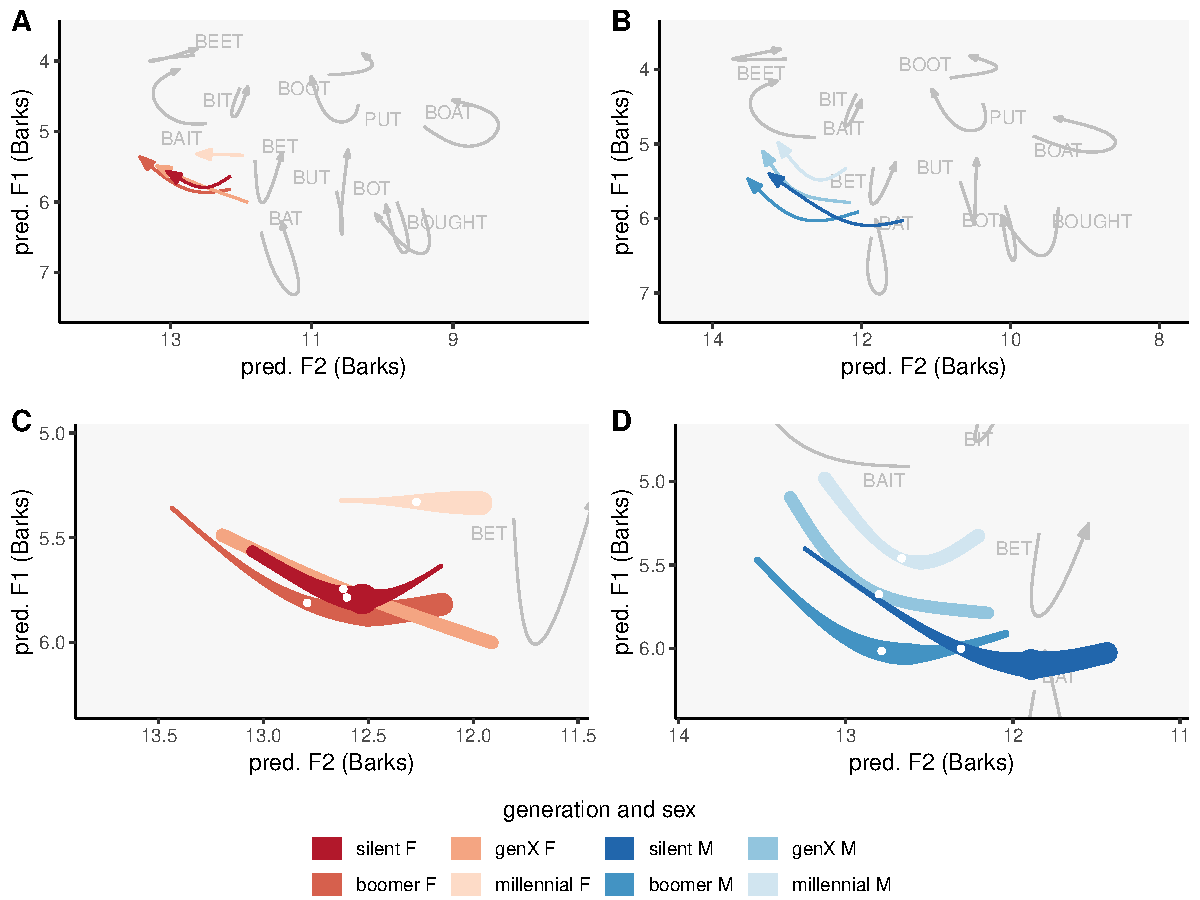
\includegraphics[width = 6.5in]{Figures/BANG/BANG_four_panel_plot.pdf}
	\caption[Predicted formant measurements for \bang by sex and generation.]{Predicted formant measurements for \bang by sex and generation. Women are on the left and men on the right. Darker shades represent older generations.}
	\label{fig:BANG_four_panel}
\end{figure*}

When the data is split up by generation (Figure~\ref{fig:BANG_four_panel}), the shape of the vowel's curve is similar across all ages, though its relative height and the degree of fronting varies in a somewhat haphazard way.\footnote{The Gen X and Millennial women's curves are perfectly straight lines. My suspicion is that there was not enough data or too much variance for the GAMM to fit a proper curve, so it generated a simple line.} Beginning with the women, we see that the older three generations do not change their realizations of \bang in an appreciable way. The shapes differ slightly, but the difference smooths suggest that they are not significant (\ref{fig:bang_diff_smooths_gen}A--B,E--F,I--J,M--N). However, like other vowels, the Millennial women exhibited the most amount of change. They had the highest, most retracted, and most monophthongal realizations of \bang. This shift was significant in F1 along most of the first half of the vowel (\ref{fig:bang_diff_smooths_gen}Q,U) and in F2 along the second half (\ref{fig:bang_diff_smooths_gen}R,V). On average, the older three generations' trajectory lengths for \bang was 1.28 Barks while for the Millennial women it barely over half that at 0.67 Barks.

The men in Cowlitz County meanwhile shifted \bang more gradually. The difference between any two consecutive generations was insignificant (\ref{fig:bang_diff_smooths_gen}C--D,O--P,W--X), but comparing the Silent men to the Millennial men, the first 20\% of the duration is primarily where the difference lies (for both F1 and F2; \ref{fig:bang_diff_smooths_gen}K--L). The pattern of monophthongization was also apparent, and occurred gradually from 2.01 Barks in the Silent men to 1.17 in the Millennials. Interestingly, as they raise the vowel, the men keep the offsets approximately in the same place while fronting the onset, resulting in that significant difference in F2. The women meanwhile keep the onset approximately the same while ending the offglide earlier, resulting in a slightly more retracted \bang.

\begin{figure*}[p]
	\centering
	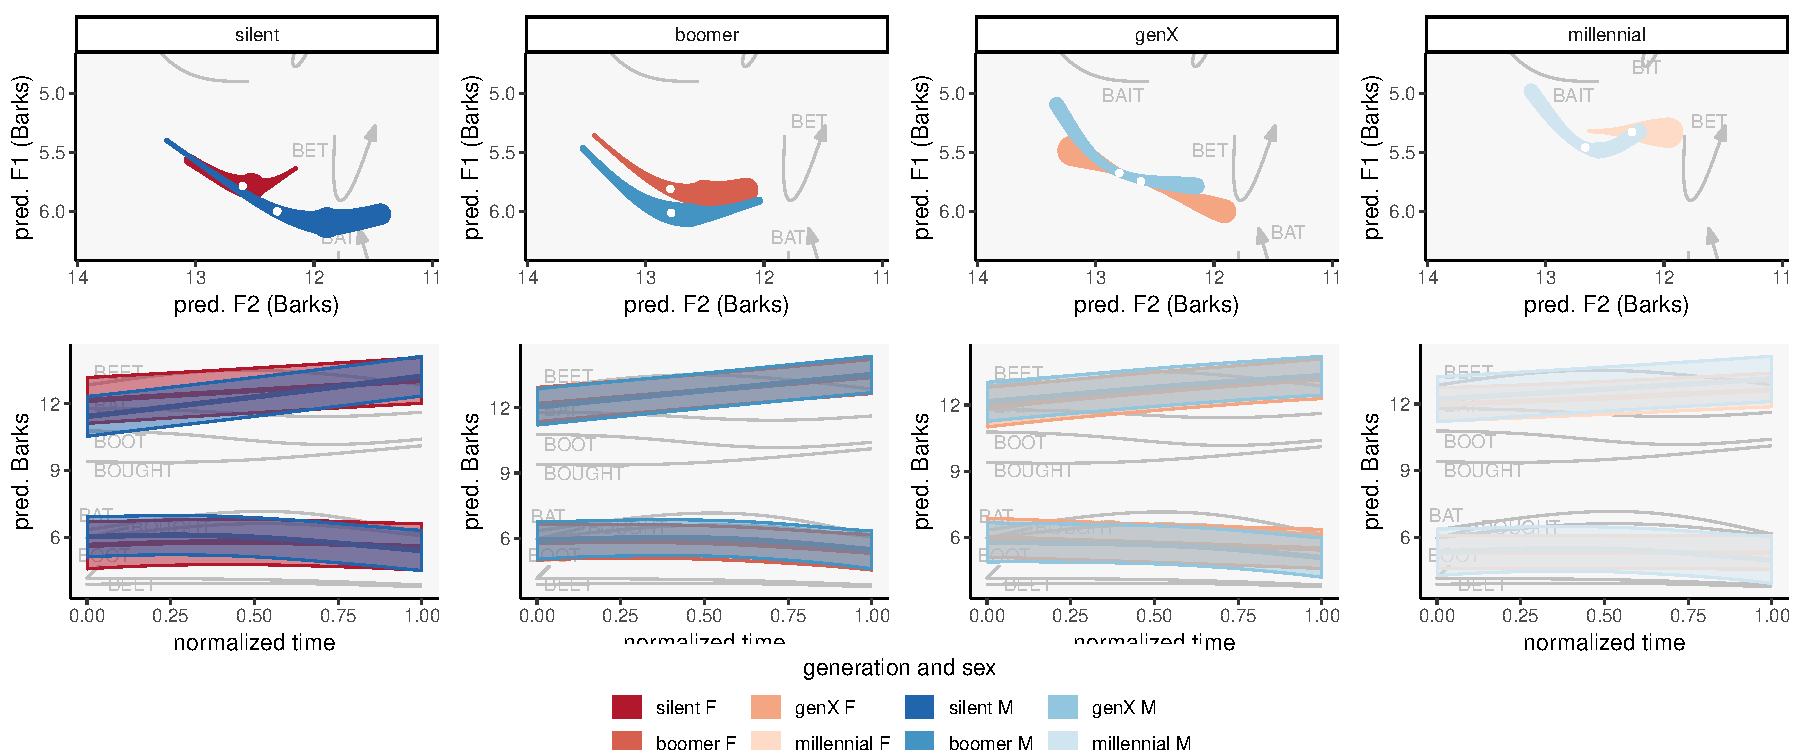
\includegraphics[angle = 90, origin = c, height = 6in]{Figures/BANG/BANG_sex_panel_plot_wide.pdf}
	\caption[Predicted formant measurements for \bang by generation.]{Predicted formant measurements for \bang by generation.}
	\label{fig:BANG_sex_panel_plot_wide}
\end{figure*}

This shift in opposite directions is more apparent in Figure~\ref{fig:BANG_sex_panel_plot_wide}, which compares men and women in the same generation. The difference between the sexes was slight and none of the difference smooths here came out significant (\ref{fig:bang_diff_smooths_sex_gen}).\footnote{The one exception was a very small portion near the onset of the F2 differences in the Silent generation, but I am hesitant to call that a meaningful difference.} So, when interpreting this pattern of men fronting \bang and women retracting it, care should be taken. The low token count likely accounts for the large confidence intervals and additional study that focuses on extracting many tokens of \bang will be necessary to substantiate this pattern.





\section{\beng}
\label{BENG}

In \S\ref{word_classes} I explain that there are very few word containing \beng in English. In a study of the front lax vowels in California, \citet[40]{cardoso_etal_2016_pads} were forced to exclude this vowel class from analysis because there was only one token from their sample of 22 speakers. In Cowlitz County, I collected only 76 tokens of \beng, though this was primarily through the ``Cat and the Mice'' passage which contained the words \textit{length} and \textit{strength}. In conversation there were an additional five tokens of \textit{lengths}, three of both \textit{length} and \textit{strength}, and one each of \textit{lengthy} and \textit{strengthen}. Because there are so few tokens (and none by Millennial men), a robust analysis of \beng using GAMMs is not possible.

\begin{figure*}[tb!]
	\centering
	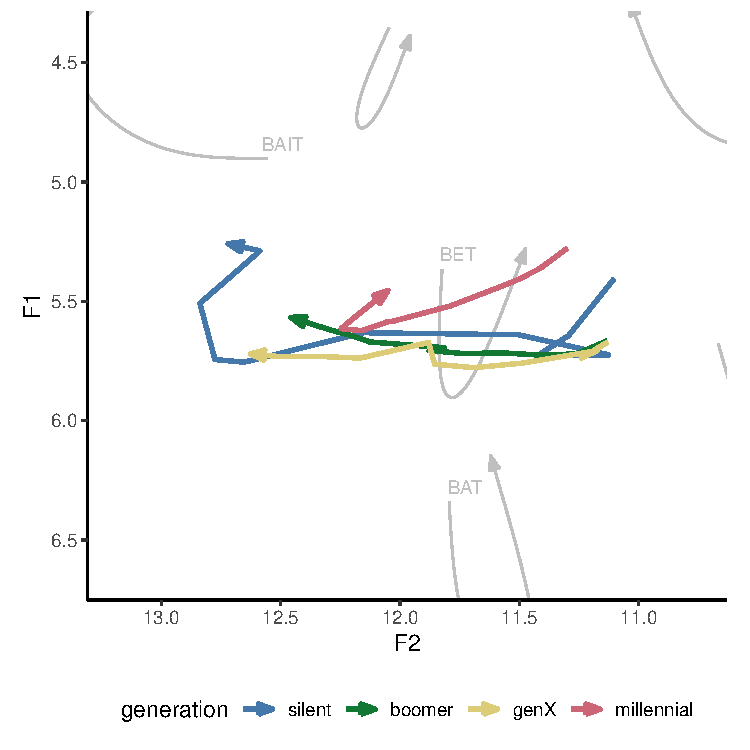
\includegraphics[width = 3.25in]{Figures/BENG/BENG_raw.pdf}
	\caption[Average trajectories for \beng by generation.]{Average trajectories for \beng by generation based on normalized formant measurements (not predicted values), transformed into Barks. Unlike every other plot in this study, this figure includes data from the reading passages.}
	\label{fig:BENG}
\end{figure*}

I can only provide a small glimpse into what this vowel is like. Figure~\ref{fig:BENG} shows the normalized values for \beng, averaged for each generation. Data from the reading passages was included because only 12 tokens of \beng occurred in conversation. This plot shows that the
\beng vowel begins with quite a low F2, but this is likely due to the fact that every token of \beng in this corpus is preceded by light /\textipa{l}/ or /\textipa{\*r}/, which are characterized by their low F2 values \citep{olive_etal_1993}. This predictable consonantal effect makes comparison with \bang and \bing difficult, at least with respect to the onset of F2. Other than this longer trajectory, \beng appears to share properties with \bang: the trajectory is primarily along the F2 dimension, it is about the same height as \bet. The offset of \beng is approximately as front as \bit while \bang goes as far front as \fleece. In IPA, \beng is [\textipa{\t{\=*{\~E}\textsubarch{\|+{\~E}}}}]: a retracted, nasalized mid-open vowel with a fronted, nasalized mid-open offset.

Without additional data, generalizations are only speculative at this point. Because their trajectories overlap in the vowel space, it is possible that \beng and \bang are merged.\footnote{Impressionistically, I do not hear a difference between \bang and \beng.} However, \beng appears slightly more centralized then \bang, both at the onset and the offset, but this may be the result of coarticulatory effects. Because of the extremely limited set of words containing \beng, additional study---possible one that analyzes the realization of nonce words with \beng---is needed to fully understand this vowel. Further analysis on this vowel in Cowlitz County will be saved for future analysis.






\section{\bing}
\label{BING}

Finally, the last vowel to be described in this chapter is \bing, or rather, \kit before velar nasals. This corpus has 2,222 tokens of \bing coming from 85 unique words. There were actually more observations of \bing than \bin, but they come from fewer tokens. The most frequent words by a large margin were \textit{think} and \textit{thing(s)}, which were followed by \textit{thinking}, \textit{bring}, \textit{single}, \textit{English}, \textit{drink}, \textit{spring}, and \textit{sing}, and \textit{ring}. There was an average of 41 tokens of \bing per person\footnote{Speakers ranged from 11 to 168 tokens with a standard deviation of 24.5: 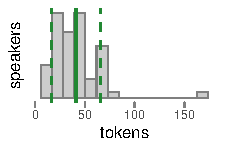
\includegraphics[width = 1.5in]{Figures/BING/BING_tiny.pdf}} for an average of 278 per generation per sex. Like \bin, this vowel exhibits relatively few changes across social groups in Cowlitz County.


% There's really no good place to put this.
\begin{figure*}[tb!]
    \centering
    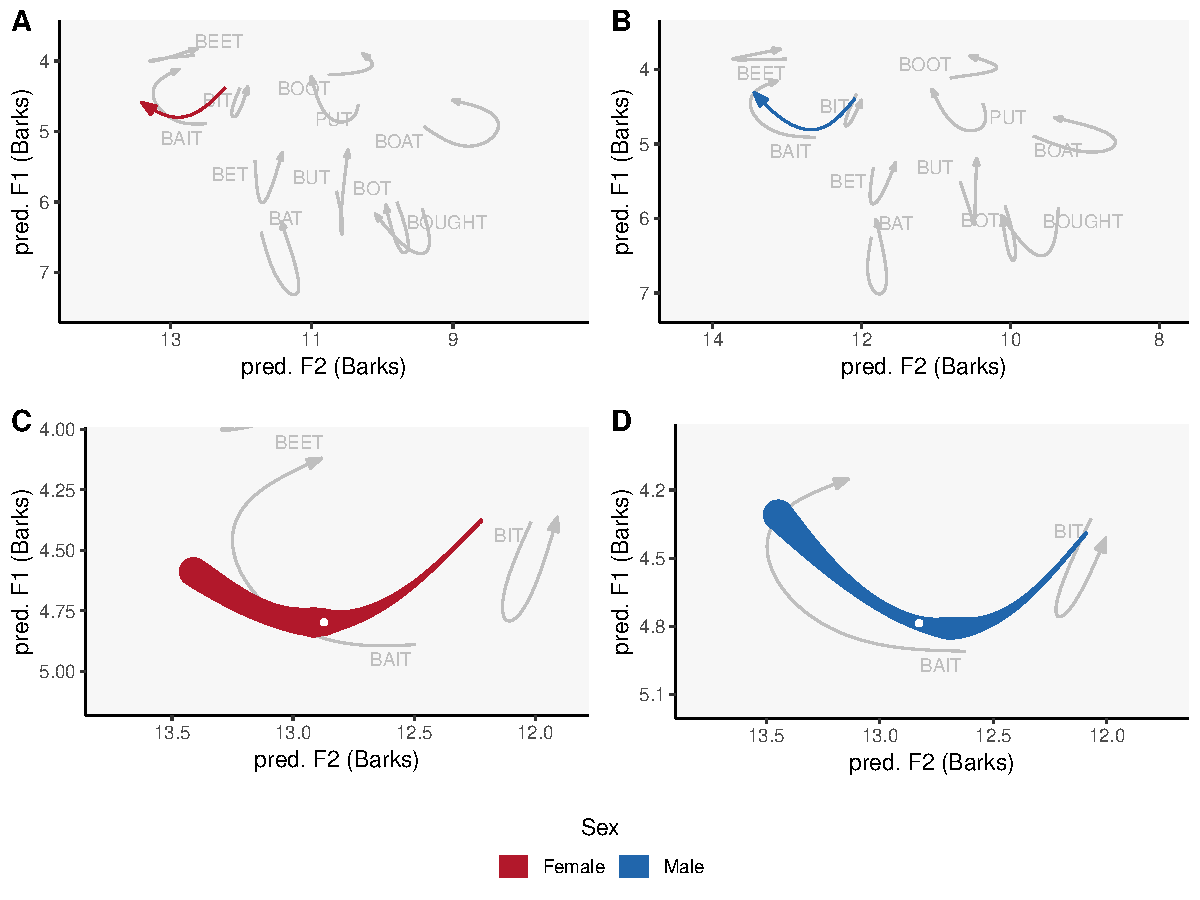
\includegraphics[width = 6.5in]{Figures/BING/BING_four_panel_plot_summarized.pdf}
    \caption[Predicted formant measurements for \bing by sex.]{Predicted formant measurements for \bing by sex with women on the left and men on the right. Predicted values are averaged across all generations.}
    \label{fig:BING_four_panel_plot_summarized}
\end{figure*}

Figure~\ref{fig:BING_four_panel_plot_summarized} shows the trajectory of \bing relative to non-nasal allophones of the other vowels. The shape of the trajectory is similar to \bang where there is a large raise in F2, reflecting the velar pinch. However, \bing has more change in F1 over its duration (and a clearer target) than \bang or \beng, making it not quite as wide of a U than \bang. For both sexes, \bing occupies nearly the same position in the vowel space as \face, which is fronter than \bit and at the same height. In IPA, this vowel is a nasalized, high front lax vowel with a fronted, nasalized, high lax offglide:  [\textipa{\t{\~I\textsubarch{\~{\|+I}}}}].

\begin{figure*}[tb!]
	\centering
	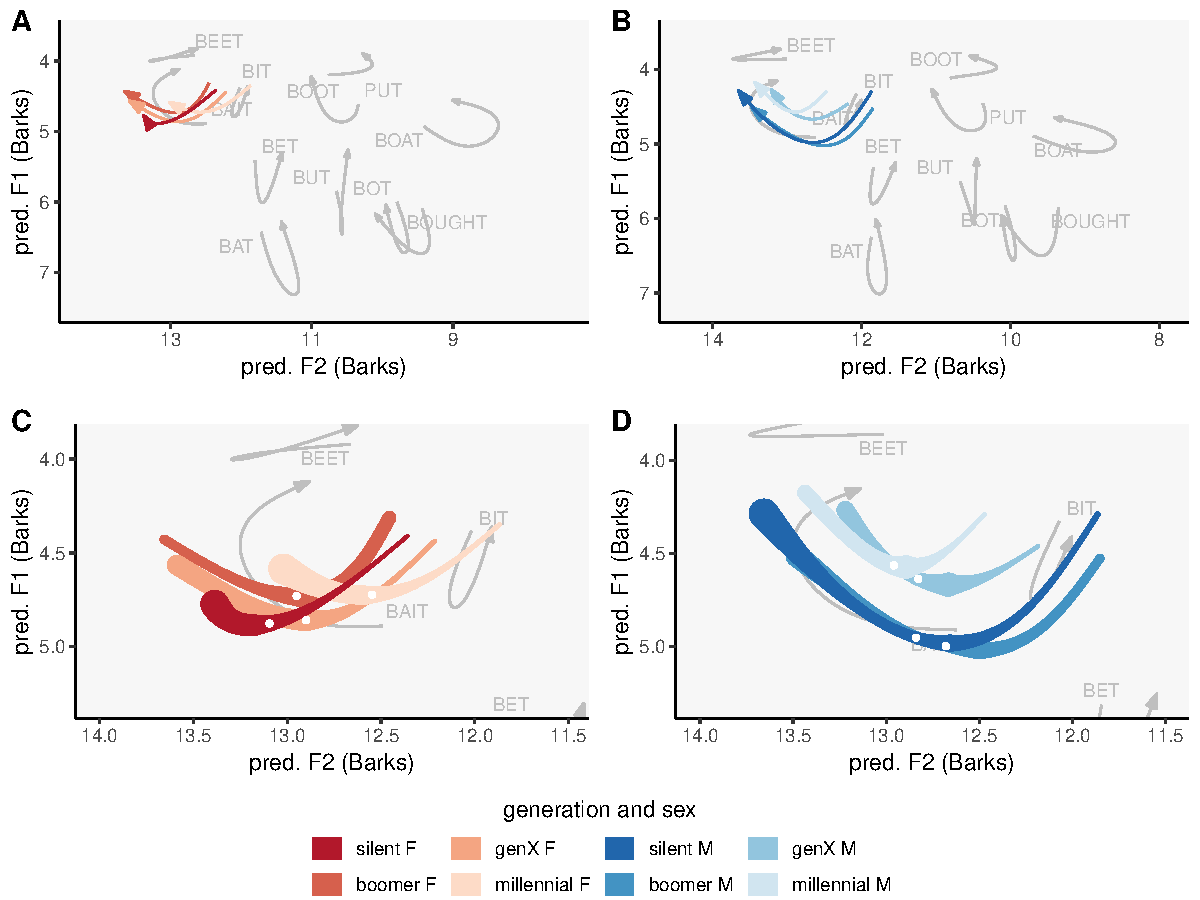
\includegraphics[width = 6.5in]{Figures/BING/BING_four_panel_plot.pdf}
	\caption[Predicted formant measurements for \bing by sex and generation.]{Predicted formant measurements for \bing by sex and generation. Women are on the left and men on the right. Darker shades represent older generations.}
	\label{fig:BING_four_panel}
\end{figure*}

When splitting the data up by generation, as in Figure~\ref{fig:BING_four_panel}, there are differences between how the women and men changed their realizations of \bing in apparent time. Beginning with the women, there is no appreciable change in height between generations, though there is some change in F2. Recall that for \bin, the women centralized the vowel slightly in apparent time while making it less diphthongal. Likewise, there was no statistical significance among the the oldest three generations' realizations of \bing at all (\ref{fig:bing_diff_smooths_gen}A--B,E--F,M--N). However, the Millennial women had the most centralized variant and difference smooths suggest that this fronting, compared to all three previous generations, is statistically significant (\ref{fig:bing_diff_smooths_gen}J,R,V). It appears that \bing is retracting in apparent time just as \bin and \bit are and that and this change may have started relatively recently.

In contrast, this backing is not found in the men's data. Figure~\ref{fig:BING_four_panel} shows that the Gen X and Millennial-aged men had a higher variant of \bing. In addition \bing gets less dynamic as trajectory lengths for the older two generations averaged 2.17 Barks while for the younger generation it was only 1.23 Barks. Difference smoooths suggest some fronting in the younger generation (\ref{fig:bing_diff_smooths_gen}L,T), but it was only in the onset of the vowel, which is more indicative of the shorter trajectory rather than fronting of the entire vowel. Compared to \bin, there is a clearer change in apparent time for men's realizations of \bing, which justifies treating these two variables separately.

\begin{figure*}[p]
	\centering
	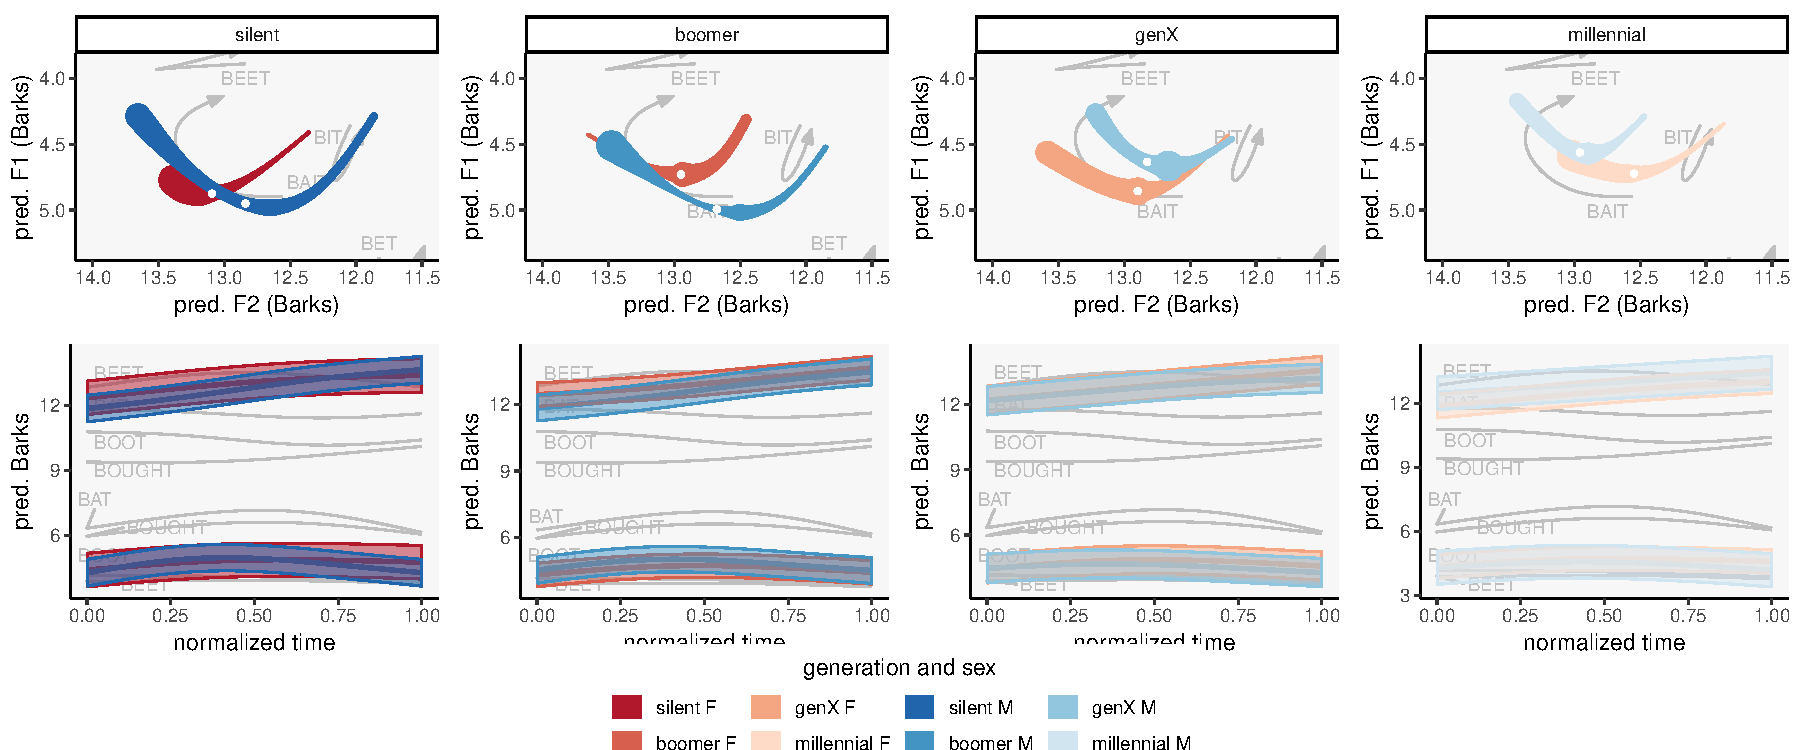
\includegraphics[angle = 90, origin = c, height = 6in]{Figures/BING/BING_sex_panel_plot_wide.pdf}
	\caption[Predicted formant measurements for \bing by generation.]{Predicted formant measurements for \bing by generation.}
	\label{fig:BING_sex_panel_plot_wide}
\end{figure*}

Finally, Figure~\ref{fig:BING_sex_panel_plot_wide} shows that the differences between the sexes within each generation is somewhat haphazard and difficult to interpret. The various difference smooths suggest a number of statistical significant difference between the sexes (\ref{fig:bing_diff_smooths_sex_gen}), but because of the reversing positions and various trajectory lengths, it is difficult to identify what the difference smooths are showing. Perhaps more data on \bing is needed to ascertain the whether these differences between the sexes are socially salient.

This section showed that there were some small changes in \bing in apparent time going in different directions for the men and the women. The women primarily used a variant of \bing similar to [\textipa{e}], except for the Millennials who used a more retracted form. Meanwhile, the older two generations of men used a lower and more diphthongal \bing while the younger two raised the vowel and shortened its trajectory.







\section{Discussion}
\label{sec:prenasal_discussion}

\subsection{Summary of findings}

The previous sections have described the trajectories of prenasal allophones of \trap, \dress, and \kit in this sample of Cowlitz County speakers.

The \ban vowel had a Bowl-shaped trajectory, starting higher and ending lower in the vowel space, fronter than \bat or \bet and somewhere between them in height. In Cowlitz County, there was a general process of raising and monophthongization in apparent time. The women in Gen X were the exception to this pattern and actually lowered the vowel quite a bit. Because the difference between the oldest two generations was not significant for either sex, Gen X appears to be the first ones to adopt \ban shifting in Cowlitz County.

Though it occupies approximately the same space as \ban, the \bang allophone had a drastically different trajectory, starting in a more centralized position and ending quite fronted as a result of the velar pinch. \bang underwent a general pattern of raising and monophthongization: in the men this was a gradual process over the four generations but in the women it starts only with the Millennials.

The trajectory of \ben was somewhat of an anomaly in this chapter, exhibiting quite a pointy shape. The oldest women used quite a fronted variant, but this gradually retracted and lowered somewhat in apparent time. Furthermore, the younger generations anticipated the peak F1 more than the older ones, shifting the timepoint of the target from 68\% of the way into the duration to 44\%. The men did not appear to shift \ben in the F1-F2 space but, like \bet, they did keep up with the women in ``smoothing'' out the trajectory shape from a bounce to more U-shaped.

A full analysis of \beng is difficult given the extremely low frequency and because all the token in this corpus had \beng following a liquid. Nevertheless, it appears that \beng is similar to \bang in position and trajectory.

\bin was slightly lower than \bit in the vowel space, and had a trajectory like a more monophthongal \ban. In apparent time, while the men did not participate in any changes, the women gradually retracted the vowel and made it more monophthongal. The amount of change from one generation to the next was small, but it appears that the Millennial-aged women shifted the most.

Finally, \bing occupies the same part of the F1-F2 space as \face and was similar in shape to the other pre-velar-nasal vowels, but there was more of a peak in F1, resulting in a clearer target. The older generations use approximately the same variants, but the Millennial women show evidence of retracting \bing while the Gen X-- and Millennial-aged men used raised and more monophthongal variants.

Summarizing these findings, we see that each vowel had its own characteristics. There were changes in height (e.g. raising for \ban, \bang, and men's \bing; lowering for \ben; no change for \bin or women's \bing) and backness (retraction in \ben, \bin, and women's \bing; no change in \ban, \bang, or men's \bing). The timing of the shift was different too. In some cases it began with Gen X (women's \ban and men's \bing) or the Millennials (women's \ban and \bing). Sometimes the change was gradual over time (men's \ban and \bang, women's \ben and \bin) and in other cases there was no change (men's \ben and \bin). In nearly every vowel though, the vowels were becoming less dynamic in apparent time.

Treating \bing and \bang as distinct allophones from \bin and \ban was justified at the very least by their different trajectories. \bang and \bing were markedly different from \ban and \bin with relatively little change in F1 but large changes in F2. In both cases, the vowels gradually fronted over the course of their trajectories, presumably as a result of the velar pinch. Both pre-/\textipa{N}/ allophones were appreciably higher than the other prenasal allophones: \bang was even more raised than \ban was while \bing shares the same F1 space as \bit. However, these differences can be attributed to coarticulatory effects.

More importantly, treating the pre-/\textipa{N}/ vowels as separate allophones uncovered social patterns that were distinct from those found in the pre-/\textipa{m}/ and pre-/\textipa{n}/ data. For example, women in Gen X used a lower and more diphthongal \ban compared to the older generations, but the same cannot be said of \bang. The younger two generations of men used higher and more monophthongal variants of \bing but not \bin. And while women are retracting \bin incrementally over the four generations, they held \bing stable until the Millennial women raised it. In other words, splitting \trap, \dress, and \kit into \ban, \bang, \ben, \beng, \bin, and \bing is justified. Furthermore the use of GAMMs to analyze them uncovers changes in trajectory that a single-point analysis would miss.





\subsection{Structural relationship between the front lax vowel allophones}

How do these prenasal allophones compare to the same vowels in other environments? Figure~\ref{fig:combined_nasal_plot} illustrates the trajectories of these vowels across all social groups, showing the position of these nasal allophones in relation to their preobstruent counterparts in the vowel space.

\begin{figure*}[p]
    \centering
    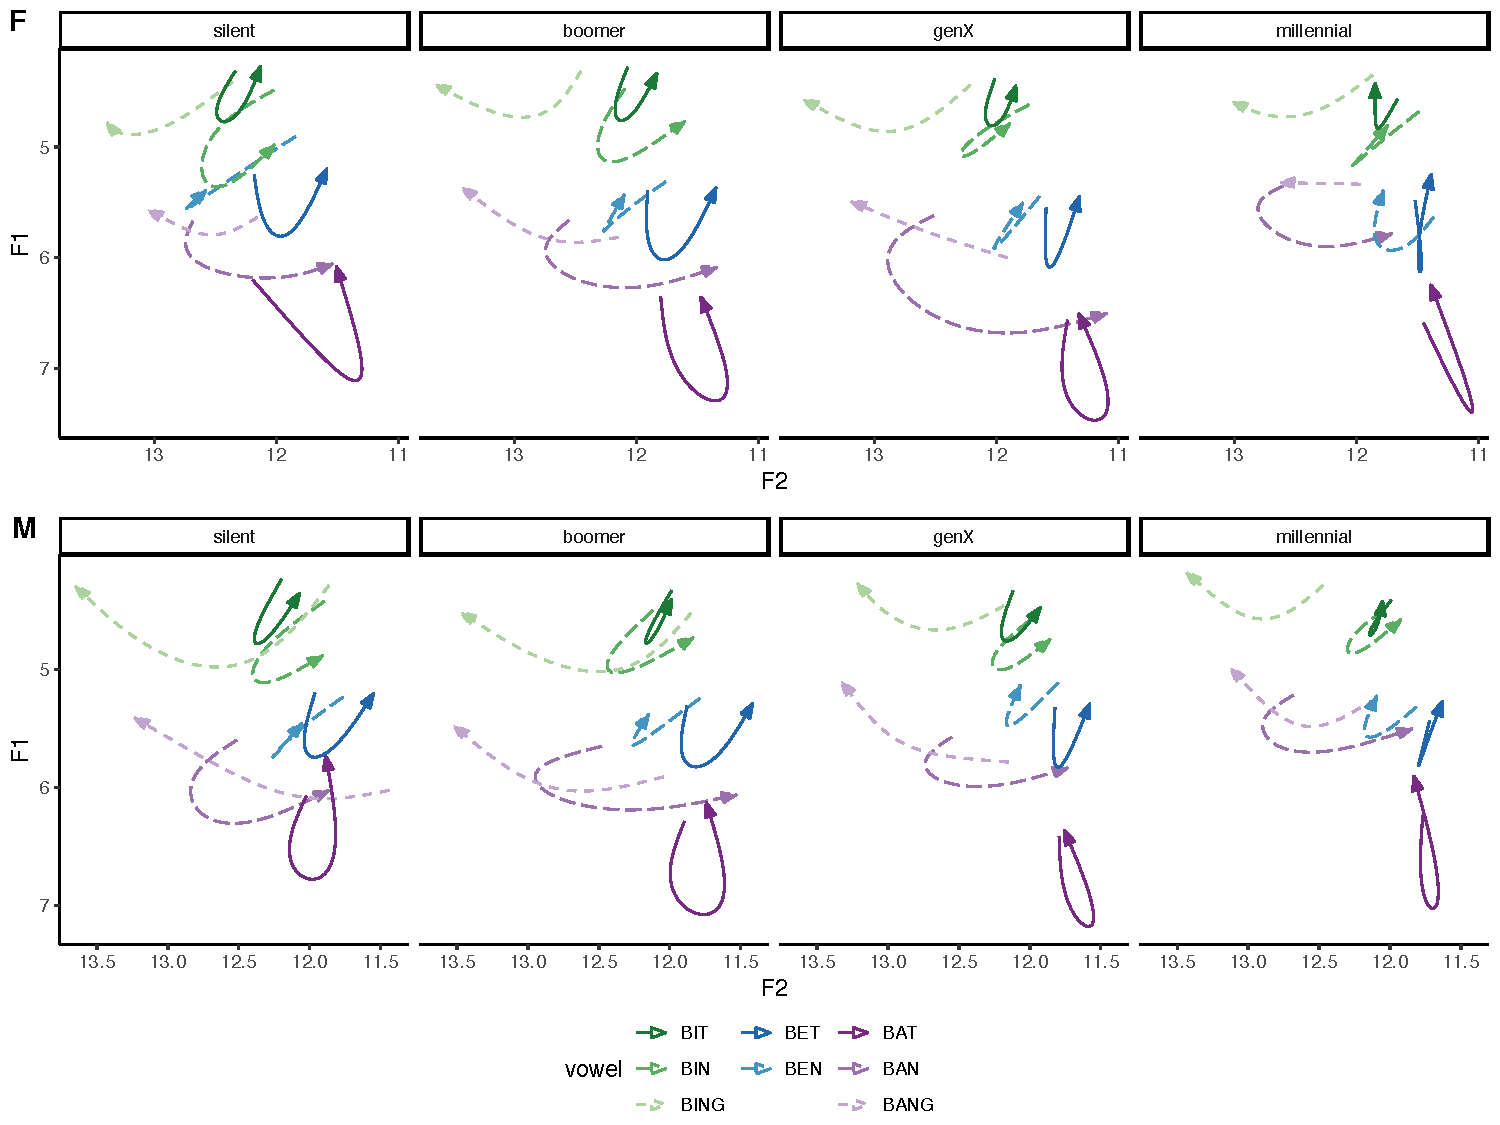
\includegraphics[angle=90, origin=c, width = 6in]{Figures/other_figures/combined_nasal_plot.pdf}
    \caption[Predicted values for all prenasal and preobstruent allophones]{Predicted values for all prenasal and preobstruent allophones of \kit, \dress, and \trap, by generation. Female values are on top and male values are on the bottom.}
    \label{fig:combined_nasal_plot}
\end{figure*}

% Relative position compared to BAT, BET, and BIT
The prenasal allophones occupied a different portion of the vowel space than the elsewhere allophones, but the direction of this difference was not consistent across the vowel classes. Beginning with \trap, it is quite clear that \ban and especially \bang are raised and fronted in relation to \bat. The distance between \ban and \bat increases in apparent time for both sexes as \bat lowers and retracts while \ban raises and fronts. However, the change in apparent time in \bang does not fit quite as nicely with \bat and \ban. Among the men, \bang appears to pattern closely with \ban as it raises gradually across the four generations. But only the Millennial women raise \bang suggesting that this is a recent adoption. Regardless, the fact that \bang is quite high and front compared to \bat supports the prenasal split in these speakers. It is clear then that the prenasal split is robust and actively spreading in Cowlitz County.

Comparing the \dress allophones, we see that \ben was more fronted than \bet, and for some people, slightly higher. But this raising is certainly not to the same degree that \ban was in relation to \bat. In fact, Figures~\ref{fig:BET_four_panel} and \ref{fig:BEN_four_panel} show that women are retracting and lowering both \bet and \ben at about the same rate, suggesting there is not a prenasal split like there is with \trap. In other words, the differences between \ben and \bet may simply be phonological rather than sociolinguistic. What does stand out is that, for both sexes, the trajectory shapes for \bet shift from a U to a Bounce while for \ben they shift from a Bounce to a U.

As for \kit, the prenasal split is not apparent since the changes in apparent time in \bit, \bin, and \bing are all similar. There is no change in height, but there is evidence of backing, except between the Boomer women and Gen X (which was true for both \bit and \bin). That the amount of shift in apparent time for \bit, \bin, and \bing was relatively small suggests that there is not a lot of meaningful sociolinguistic change happening with respect to these vowels and that the differences between them are simply phonological.

For all vowels there was a complex interaction between sex and generation, many of which involving a change in apparent time. This interaction suggests that prenasal variants are quite volatile, but given that the overall differences between the oldest and the youngest generations were relatively small for some allophones of \dress and \kit, the speech of this community does not appear to be undergoing major changes for all vowels. Therefore, it is not the case that all three prenasal allophones are raised in comparison to the preobstruent allophones. In other words, this trajectory data in Cowlitz County supports what \citep{cardoso_etal_2016_pads} find in San Francisco, namely that the nasal split only applies to \trap.

% Relationship between the prenasal allophones only

\begin{figure*}[tb!]
    \centering
    \hspace{\fill}
     \begin{subfigure}[t]{2.925in}
        \centering
        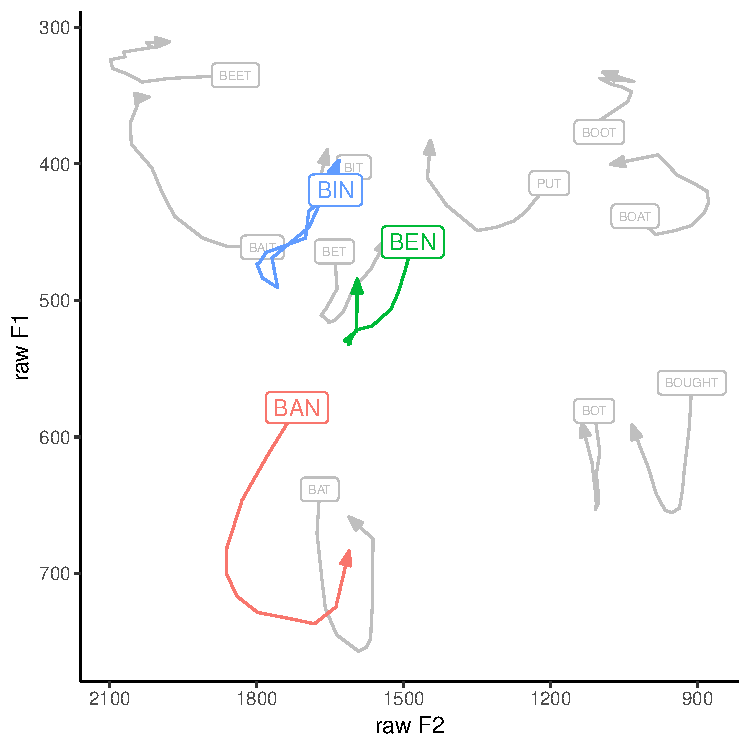
\includegraphics[width = \textwidth]{Figures/example_plots/07-Anthony_avg_prenasal.pdf}
        \caption{Anthony's prenasal vowels.}
        \label{fig:anthony_prenasal}
    \end{subfigure}
    \hspace{\fill}
    \begin{subfigure}[t]{2.925in}
        \centering
        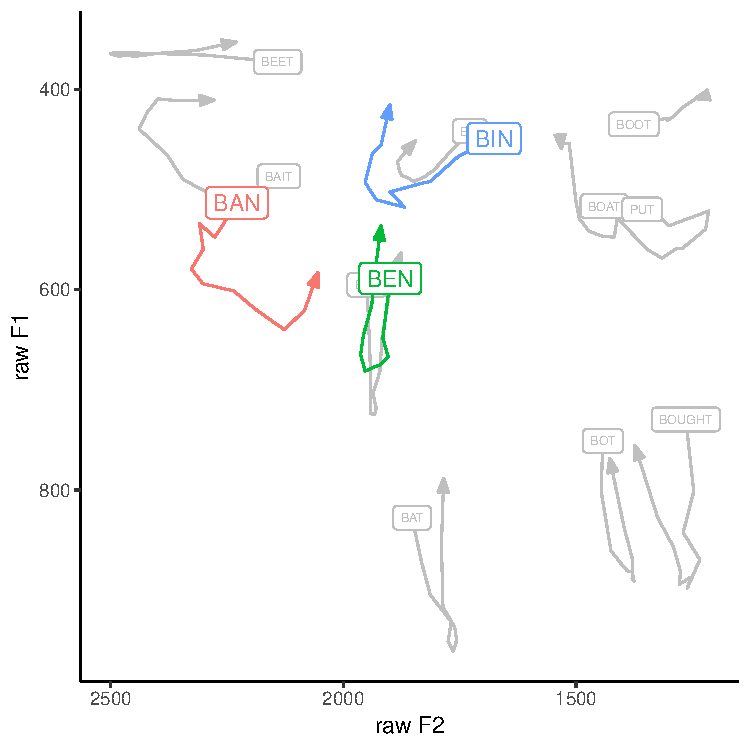
\includegraphics[width = \textwidth]{Figures/example_plots/05-Megan_avg_prenasal.pdf}
        \caption{Megan's prenasal vowels.}
        \label{fig:megan_prenasal}
    \end{subfigure}
    \hspace{\fill}
    \caption{Sample plots showing conservative and innovative \ban variants.}
    \label{fig:anthony_and_megan}
\end{figure*}

In fact, because the prenasal allophones are shifting in different directions, we find that they  are arranged quite differently in relation to each other than their preobstruent counterparts are. The Millennials are raising \ban such that \ban and \ben are at approximately the same height. Figure~\ref{fig:anthony_prenasal} shows the average trajectories for Anthony, a man born in Cowlitz County in 1954. His conservative realization of \ban is quite low and overlaps with \bat. Meanwhile, Figure~\ref{fig:megan_prenasal} shows that Megan, who was born in 1992, uses a very high variant of \ban. Its onset is comparable to that of \face, and the trajectory on average is a little higher than either \bet or \ben. Thus, while the preobstruent allophones roughly share the same F2, \ban and \ben are primarily differentiated by their F2. It should be noted though that for Megan and others with a very high \ban vowel, there is likely no threat of a merger with \ben because the two vowels are separated by a relatively wide margin along F2 and because the trajectories go in opposite directions.

This difference in trajectory found in \ben is noteworthy. Figure~\ref{fig:combined_nasal_plot} shows that, in general, the three vowels share the same trajectory shape in the environments in the previous and the current chapter. Recall that \bat, \bet, and \bit have generally the same inward-hooking U-shaped trajectory. \bang, \bing, and (so far as we can tell) \beng also have a similar shape as a result of the velar pinch. However, while \ban and \bin share a resemblance with their Bowl-shaped curve, \ben's trajectory is a bit of a misfit. It is either a narrow V or it is an outward-hooking U with the offset fronter than the onset (the opposite direction from \ban and \bin). To my knowledge, there are no other studies on \ben in the West that incorporate trajectory shape, so it is impossible to tell whether this is a more widespread trend or if it is unique to this community.

Concluding this section, the structural relationship between the prenasal allophones of \trap, \dress, and \kit is weak. The vowels differ in their trajectory shape and shift in different directions. The link between \bing, \beng, and \bang appears somewhat stronger, but this is likely a result of the strong coarticulatory effects of the following velar nasal. The link between \bin, \ben, and \ban is virtually non-existent. Though \bit, \bet, and \bat appear to be connect and are shifting together, their prenasal counterparts do not form a cohesive group and the movement of one does not appear to influence another. In other words, the prenasal allophones are more structurally (and phonologically) related to their preobstruent counterparts than with each other, with the exception of \ban which is shifting independently of \bat.

\subsection{Cowlitz County's place in the West}
\label{sec:cowlitz_place_in_west_prenasal}

The description of Cowlitz County vowels in this study closely matches the descriptions of other communities in the West---it is a characteristically western vowel pattern. In particular, \ban is as it is described in California \citep{eckert_2008, cardoso_etal_2016_pads}, Oregon \citep{becker_etal_2016_pads}, and Seattle \citep{swan_2016_diss}: a high onset and a centralized glide, with more raising in younger speakers. Because \ban-raising is such widespread shift in North American English \citep{thomas_2001}, it comes as no surprise that Cowlitz County would pattern with nearby areas.

Regarding the timing of these shifts, there are some similarities with the patterns found in other areas. The oldest two generations used similar realizations of \ban, women in Gen X used lower forms, and women Millennials used higher forms. It is reasonable to conclude that \ban was stable until roughly 1966 when Gen X started. Then, starting perhaps around 1980, \ban raised. For \bang, only the Millennial women raised it, so \bang-raising began around 1980 as well. In San Francisco, \citet{cardoso_etal_2016_pads} find that white speakers are raising \ban,\footnote{From that study alone, it is difficult to make direct comparisons with the current study because it is not clear whether the raising in San Francisco is consistent across all age groups or if one group in particular is leading the change. Here, I included generation as a categorical variable to model change in apparent time. However, \citet{cardoso_etal_2016_pads} treated age as a continuous variable and fit it to a linear mixed-effects regression model. The constraints in a linear model are such that age is modeled with a fixed slope, implying consistent and gradual shift from the oldest to youngest speakers---regardless of whether the data show a constant rate of change. If there was a period of stability followed by sudden raising (as there is in Cowlitz County) a model with age as a linear predictor would not adequately capture that pattern.} which is consistent with the findings presented here. They also find that young males are raising \bang to meet the already high variants used by the women; in Cowlitz County, the males are gradually raising \bang and only the Millennial women used high forms. So the interaction between age and sex with respect to the height of \bang was not the same in the two studies. Therefore, despite the fact that \bat lowering has been occurring in Cowlitz County since possibly the 1920s (see \S\ref{sec:cowlitz_place_in_west_preobstruent}) it appears that these same speakers have only relatively recently adopted \ban- and \bang-raising since only the Millennials show a consistent raising pattern. Since there was some indication of raising in San Francisco before 1980, it appears that the raising of prenasal allophones of \trap has spread northward from California into Washington, or at least, that it was adopted in California before it was adopted in Cowlitz County.

For \ben and \bin, Cowlitz County is different with what is reported in other areas. While  \citet{holland_2014_diss} finds that \ben was raising in California, this data support what \citet{cardoso_etal_2016_pads} find in San Francisco: that \ben and \bin are shifting together with \bet and \bit, respectively. Despite some indication of the \textit{pin-pen} merger among some speakers in the Seattle area \citep{scanlon_wassink_2010}, there is no indication of \bin and \ben approaching a merger in Cowlitz County.

For the pre-/\textipa{N}/ vowels, there is less work available for comparison in the West. \citet[46]{conn_2000_diss} finds that some speakers in Portland raise \ban higher than \bang. At least at the community level, this is not the case in Cowlitz County, and \bang was consistently higher than \ban. However, \citet{conn_2000_diss} also finds that \bang is fronter than \ban, which matches was found in Cowlitz County. Similarly, \citet[42]{cardoso_etal_2016_pads} find that \bing was higher than both \bit and \bin. This phenomenon was noted relatively early in California English, leading to descriptions such as, ``\textit{think} sounds like \textit{theenk}'' \citep{eckert_2004}. In this sample, \bing was raised, though not to the extent of overlapping with \fleece (see Figure~\ref{fig:BING_four_panel}). Likewise \citet{cardoso_etal_2016_pads} find a significant age effect on \bang, with younger speakers using higher variants, which is paralleled in Cowlitz County.

Therefore, with respect to their prenasal vowels, speakers in Cowlitz County appear to match what is found in other areas of the West, particularly San Francisco. I know of no direct connection between these regions, so it is unlikely that the patterns found here are unique to just San Francisco and Cowlitz County. Instead, it is likely that other speakers in Washington, Oregon, and  areas in the Inland West would exhibit the same prenasal system described in this chapter.


\subsection{Trajectories and prenasal allophones}

Finally, it is worth discussing the merit of studying prenasal vowels' trajectories rather than single pair of measurements. Is it worth the complexity, and if so, what additional insight can be gained by using GAMMs (or some other technique) to study vowel trajectories?

One important benefit of using GAMMs on this data (and in general) is the ability to produce difference smooths. Visualization in the F1-F2 space are excellent, but can be potentially misleading since their interpretation can be subjective. Difference smooths allow for an objective way to compare two curves and to find out not only if they are significantly different but also at what portion of the duration this significance can be found. These difference smooths are crucial when identifying significant change from one generation to the next.

One of the more practical issues is that studying the full trajectory eliminates the need for selecting a single (potentially arbitrary) point to represent the entire vowel. For the preobstruent allophones, there was a clear indication of the vowel's ``target,'' which is the result of F1 peaking somewhere in the vicinity of the midpoint, sometimes accompanied by a low point in F2 at the same time. Measurements at that point along may be justified, so long as the target is representative of how humans perceive the vowel. On the other hand, for most of the prenasal vowels a clear target is harder to identify. Consider the various realizations of \ban illustrated Figure~\ref{fig:combined_nasal_plot}. Its diphthongal Bowl-shaped pattern and lack of a steady state makes it difficult to select a representative point. This shape is a result of F1 and F2 peaking at different points: depending on the sex and generation, F1 peaks between 66\% and 75\% into the duration of the vowel and F2 peaks between 18\% and 36\% into the duration. Are one of these time points representative of \ban? Or is the midpoint, which lies approximately between these two peaks, better? I argue that at least all three are needed, and perhaps more, to adequately understand \ban. In fact, a reexamination of Figure~\ref{fig:kim_and_holly} more clearly shows two targets in Kim and Holly's \ban, rather than just one.\footnote{If I had set \textit{k} to a higher value in the GAMM, these sharper targets might have been more apparent in the predicted values. As explained in \S\ref{gamms_in_this_study} though, this extra wiggliness was not needed.} Furthermore, it suggests that even these three points would miss on the height of the onset and the centralization of the offset.

\begin{table*}[tb!]
    \caption[Trajectory length, duration, and spectral rate of change]{Three acoustic measurements for each vowel. Trajectory length (TL) is measured based on the predicted values for each sex and generation, averaged together, in Barks. Duration is based on the original raw data set and was calculated by taking the mean log duration, rescaled back into seconds. Spectral rate of change (ROC) is simply the trajectory length divided by the duration; because Barks per second is difficult to interpret, I divided by 10 to give Barks per 100 milliseconds which I feel is a more interpretable number because it more closely matches the actual durations. \beng is excluded because it was not modeled.}
    \centering
    \liningnums{
        \begin{tabular}{l r r r}
            vowel &
            \shortstack[c]{TL\\ \footnotesize{(Barks)}} &
            \shortstack[r]{duration \\ \footnotesize{(seconds)}} &
            \shortstack[r]{ROC \\ \footnotesize{(Barks per 100ms)}} \\
            \hline
            \bat  & 2.185 & 0.126 & 1.734 \\
            \ban  & 2.243 & 0.113 & 1.990 \\
            \bang & 1.394 & 0.066 & 2.104 \vspace{0.5em}\\
            \bet  & 1.470 & 0.077 & 1.906 \\
            \ben  & 1.261 & 0.062 & 2.022 \\
            \beng &   --- &   --- &    --- \vspace{0.5em}\\
            \bit  & 1.087 & 0.062 & 1.751 \\
            \bin  & 1.822 & 0.064 & 2.858 \\
            \bing & 2.015 & 0.064 & 3.142 \\
        \end{tabular}
    }

    \label{tab:spectral_rate_of_change}
\end{table*}

This issue is further problematic with the pre-/\textipa{N}/ vowels. The target is even less clear than the other prenasals. This lack of a precise point of measurement is exacerbated when the spectral rate of change\footnote{The spectral rate of change is calculated by taking the trajectory length and dividing it by the duration \citep{fox_jacewicz_2009, farrington_etal_2018}. In this case, the trajectory length was calculated as the sum of the distances between predicted measurements at 501 points along the duration of the vowel. The duration was calculated as the mean log duration per vowel (using the raw dataset), converted back into seconds.} is considered (Table~\ref{tab:spectral_rate_of_change}). \bing and \bang traverse much of the F2 space, giving them long trajectory lengths, but they have relatively short durations so their spectral rate of change is high. However, because \bat is an especially long vowel\footnote{The duration of \bat is in fact the longest of the monophthongs in Cowlitz County \citep[cf.][]{peterson_lehiste_1960}.} its rate of change is much lower. That is to say that \bang is a faster moving target, and small deviations in the time point from which formant measurements are estimated will have larger effects on the results. This is easily overcome if the full trajectory is analyzed.

Another justification for using GAMMS in this study is that trajectories differences are more easily detected with them. Recall that in \S\ref{sec:trajs_and_elsewhere_shift} I show the gradual ``tightening up'' of the preobstruent vowels as they shift from a U-shape to a Bounce, meaning F2 is more stable. The main finding with the prenasal vowels is that while \bin and \ban are ingliding vowels (F2 lowers over their duration), \ben goes the opposite way (F2 generally raises over its duration). There is no obvious articulatory motivation: the majority of the most common \ben words contain an /\textipa{n}/ rather than an /\textipa{m}/, and which generally cause a small drop in both F1 and F2 \citep[143, 193]{olive_etal_1993}. The model predictions do reflect the raw data though: Figure~\ref{fig:marilyn_and_earl} shows two speakers and their left-hooking \ben vowel. In the left (Figure~\ref{fig:marilyn_prenasal}) is Marilyn, a woman born in 1950 and on the right (Figure~\ref{fig:earl_prenasal}) is Earl, a man born in 1946; both speakers exemplify the left-hooking trajectory of \ben. I have no firm explanation for why \ben hooks left while the other vowels were not predicted to do so, though one hypothesis is that \ben's target is a centralized vowel and that part of its vowel-inherent spectral change is the front offglide. The important part is that the GAMMs were able to capture this pattern; I leave it for future study to find potential social salience in these differences.

\begin{figure*}[tb!]
    \centering
    \hspace{\fill}
    \begin{subfigure}[t]{2.925in}
        \centering
        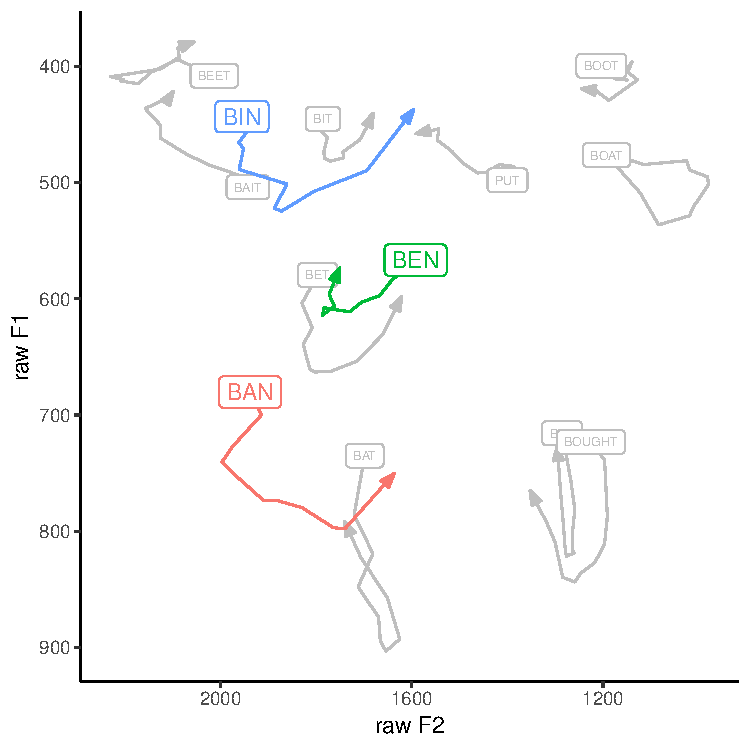
\includegraphics[width = \textwidth]{Figures/example_plots/37-Marilyn_avg_prenasal.pdf}
        \caption{Marilyn's prenasal vowels.}
        \label{fig:marilyn_prenasal}
    \end{subfigure}
    \hspace{\fill}
    \begin{subfigure}[t]{2.925in}
        \centering
        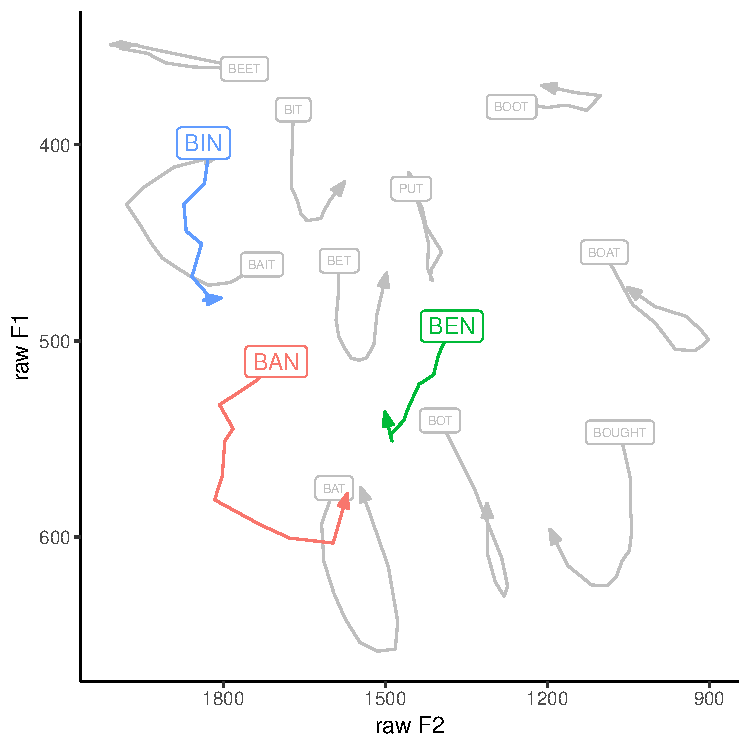
\includegraphics[width = \textwidth]{Figures/example_plots/16-Earl_avg_prenasal.pdf}
        \caption{Earl's prenasal vowls.}
        \label{fig:earl_prenasal}
    \end{subfigure}
    \hspace{\fill}
    \caption{Average trajectories (in normalized Hz) for two people showing the left-hooking \ben trajectory.}
    \label{fig:marilyn_and_earl}
\end{figure*}



The other pattern that was found using GAMMs was that the timepoint in which F1 was at its peak got progressively earlier in apparent time, particularly for \ben. Figure~\ref{fig:change_in_nucleus} shows the timepoint for the max F1 for most of the vowels in this chapter. There is some shift in apparent time in all groups, but there is a general trend of anticipating when F1 is at its maximum (as evident by the downawrd sloping lines). This is most noticeable in  \bet, \ben, and \bin, but the slope is the greatest (indicating the most amount of change in apparent time) with \ben. This anticipation is actually possible to detect using single-point measurements alone, if the heuristics for when to extract formant measurements is dependent on peak F1\footnote{FAVE does extract formant measurements at the peak F1 for \face and \price and halfway between the onset and the peak F1 for \goat, and \mouth\citep[35]{labov_etal_2013}. However, relative position of formants are not considered for \dress (and therefore \ben).}. However, with noisy audio and Praat's imperfect formant estimator, the peak F1 may be an erroneous measurement. Extracting measurements at many more time points and then smoothing them out with GAMMs is potentially a more reliable method for tracking this kind of shift.

\begin{figure*}[tb!]
    \centering
    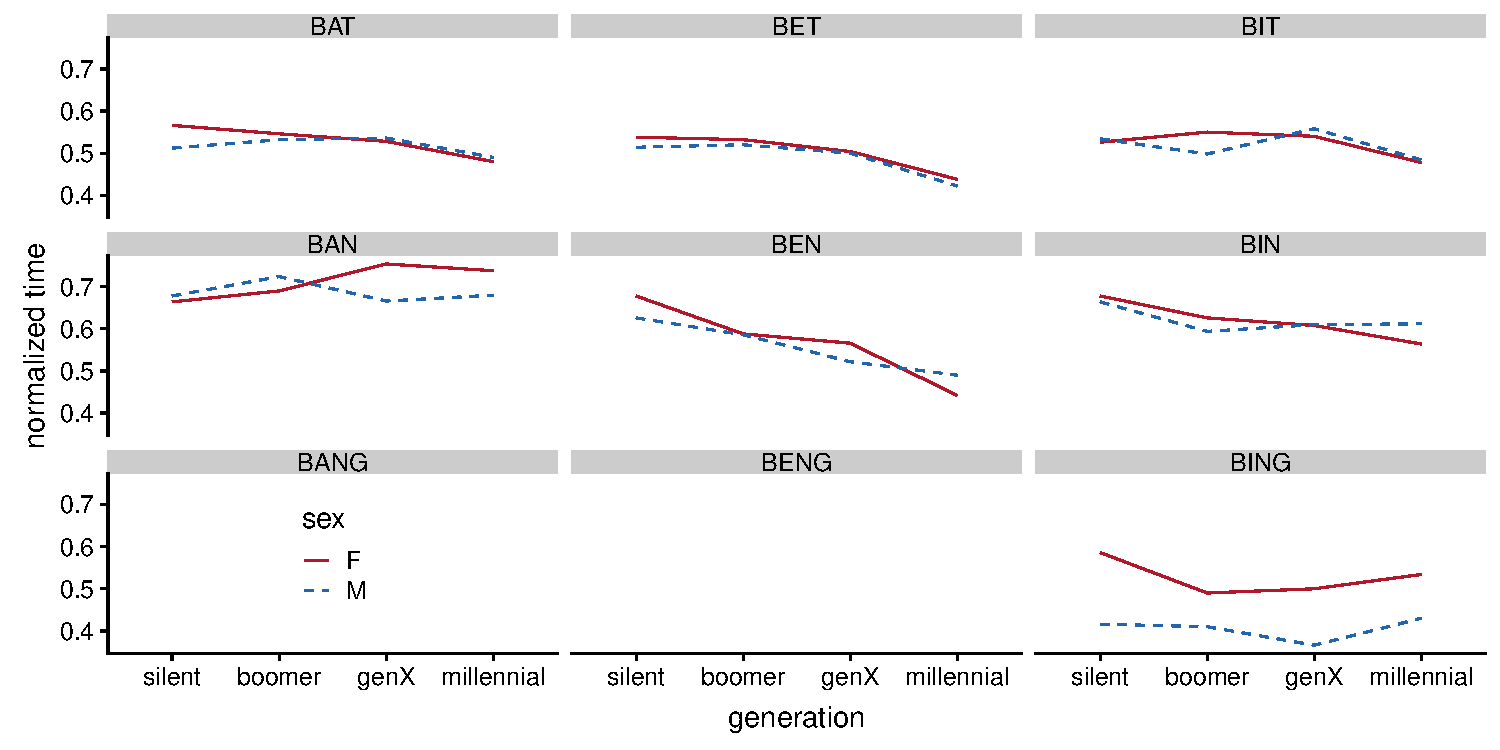
\includegraphics[width = 6.5in]{Figures/other_figures/change_in_nucleus.pdf}
    \caption[Peak F1 timepoints]{Peak F1 timepoints. \beng was excluded because it was not modeled and \bang was excluded because F1 was at its highest at the onset in Gen X.}
    \label{fig:change_in_nucleus}
\end{figure*}

The last finding that GAMMs proved effective in illuminating was the monophthongization in many of the prenasal vowels in apparent time. There are other methods for quantifying how monophthongal or diphthongal a vowel is. \citet{morrison_2013}, \citet{jacewicz_etal_2006}, and \citet{farrington_etal_2018} demonstrate a variety of these methods, some of which were adapted and used in this chapter to quantify the visual patterns in the plots. Nevertheless, I believe the output of the GAMMs produced more convincing and detailed visualizations in a way that a less gradient method could not.

Therefore, the use of GAMMs was justified in the study of prenasal allophones. It eliminated an arbitrary selection of time point, facilitates the analysis of very dynamic vowels, and illuminates trajectory differences. It also makes it easier to spot a shifting target timepoint and to visualize monophthongization.

\section{Conclusion}
\label{sec:prenasal_conclusion}

This chapter examined prenasal allophones of \trap, \dress, and \kit in Cowlitz County, Washington, with an emphasis on their trajectories. Unlike their preobstruent counterparts, there is little evidence of a structural relationship between these vowels. The vowels all move in different directions, at different rates, and starting at different times. The Millennial women exhibit the most amount of change compared to the generation previous. The most widespread commonality in these vowels is a trend towards more monophthongal realizations in apparent time. Each of these patterns is supported and exemplified by examining raw data from individual speakers. In conclusion, the prenasal split, when applied to \trap only, is active and robust in Cowlitz County.
